% XeLaTeX document
\documentclass[12pt,a4paper]{article}
% Редактируем: конфигурация, личные настройки: имя, название предмета и пр. для титульной страницы и метаданных документа здесь
\newcommand{\university}{Санкт-Петербургский политехнический университет Петра Великого}
\newcommand{\faculty}{Институт компьютерных наук и технологий}
\newcommand{\department}{Высшая школа интеллектуальный систем и суперкомпьютерных технологий}
\newcommand{\city}{Санкт-Петербург}
\newcommand{\docname}{Отчёт по лабораторным работам}
\newcommand{\subject}{Телекоммуникационные технологии}
\newcommand{\tutorname}{Н. В. Богач}
\newcommand{\studentname}{С. А. Федоров}
\newcommand{\group}{3530901/90201}

% Не редактируем: используемые пакеты
% настройка кодировки, шрифтов и русского языка
\usepackage{fontspec}
\usepackage{polyglossia}

% рабочие ссылки в документе
\usepackage{hyperref}

% графика
\usepackage{graphicx}
\usepackage{tikz}

% поворот страницы
\usepackage{pdflscape}

% качественные листинги кода
\usepackage{minted}
\usepackage{lstfiracode}

\usepackage{listings}


\usepackage{xcolor}
%New colors defined below
\definecolor{codegreen}{rgb}{0,0.6,0}
\definecolor{codegray}{rgb}{0.5,0.5,0.5}
\definecolor{codepurple}{rgb}{0.58,0,0.82}
\definecolor{backcolour}{rgb}{0.95,0.95,0.92}

%Code listing style named "mystyle"
\lstdefinestyle{mystyle}{
  backgroundcolor=\color{backcolour}, commentstyle=\color{codegreen},
  keywordstyle=\color{magenta},
  numberstyle=\tiny\color{codegray},
  stringstyle=\color{codepurple},
  basicstyle=\ttfamily\footnotesize,
  breakatwhitespace=false,         
  breaklines=true,                 
  captionpos=b,                    
  keepspaces=false,                 
  numbers=left,                    
  numbersep=5pt,                  
  showspaces=false,                
  showstringspaces=false,
  showtabs=false,                  
  tabsize=2
}



% отключение копирования номеров строк из листинга, работает не во всех просмотрщиках (в Adobe Reader работает)
\usepackage{accsupp}
\newcommand\emptyaccsupp[1]{\BeginAccSupp{ActualText={}}#1\EndAccSupp{}}
\let\theHFancyVerbLine\theFancyVerbLine
\def\theFancyVerbLine{\rmfamily\tiny\emptyaccsupp{\arabic{FancyVerbLine}}}

% библиография
\bibliographystyle{templates/gost-numeric.bbx}
\usepackage{csquotes}
\usepackage[parentracker=true,backend=biber,hyperref=true,bibencoding=utf8,style=numeric-comp,language=auto,autolang=other,citestyle=gost-numeric,defernumbers=true,bibstyle=gost-numeric,sorting=ntvy]{biblatex}

% установка полей
\usepackage{geometry}

% нумерация картинок по секциям
\usepackage{chngcntr}

% дополнительные команды для таблиц
\usepackage{booktabs}

% для заголовков
\usepackage{caption}
\usepackage{titlesec}
\usepackage[dotinlabels]{titletoc}

% разное для математики
\usepackage{amsmath, amsfonts, amssymb, amsthm, mathtools}

% водяной знак на документе, см. main.tex
\usepackage[printwatermark]{xwatermark}

% Не редактируем: параметры используемых пакетов и не только
% настройки polyglossia
\setdefaultlanguage{russian}
\setotherlanguage{english}

% локализация
\addto\captionsrussian{
	\renewcommand{\figurename}{Рисунок}%
	\renewcommand{\partname}{Глава}
	\renewcommand{\contentsname}{\centerline{Содержание}}
	\renewcommand{\listingscaption}{Листинг}
}

% основной шрифт документа
\setmainfont{CMU Serif}
\newfontfamily\cyrillicfont{CMU Serif}[Script=Cyrillic]

% перечень использованных источников
\addbibresource{refs.bib}

% настройка полей
\geometry{top=2cm}
\geometry{bottom=2cm}
\geometry{left=2cm}
\geometry{right=2cm}
\geometry{bindingoffset=0cm}

% настройка ссылок и метаданных документа
\hypersetup{unicode=true,colorlinks=true,linkcolor=red,citecolor=green,filecolor=magenta,urlcolor=cyan,
	pdftitle={\docname},
	pdfauthor={\studentname},
	pdfsubject={\subject},
	pdfcreator={\studentname},
	pdfproducer={Overleaf},
	pdfkeywords={\subject}
}

% настройка подсветки кода и окружения для листингов
\usemintedstyle{colorful}
\newenvironment{code}{\captionsetup{type=listing}}{}

% шрифт для листингов с лигатурами
\setmonofont{FiraCode-Regular.otf}[
	SizeFeatures={Size=10},
	Path = templates/,
	Contextuals=Alternate
]

% оформления подписи рисунка
\captionsetup[figure]{labelsep = period}

% подпись таблицы
\DeclareCaptionFormat{hfillstart}{\hfill#1#2#3\par}
\captionsetup[table]{format=hfillstart,labelsep=newline,justification=centering,skip=-10pt,textfont=bf}

% путь к каталогу с рисунками
\graphicspath{{fig/}}

% Внесение titlepage в учёт счётчика страниц
\makeatletter
\renewenvironment{titlepage} {
	\thispagestyle{empty}
}
\makeatother

\counterwithin{figure}{section}
\counterwithin{table}{section}

\titlelabel{\thetitle.\quad}

% для удобного конспектирования математики
\mathtoolsset{showonlyrefs=true}
\theoremstyle{plain}
\newtheorem{theorem}{Теорема}[section]
\newtheorem{proposition}[theorem]{Утверждение}
\theoremstyle{definition}
\newtheorem{corollary}{Следствие}[theorem]
\newtheorem{problem}{Задача}[section]
\theoremstyle{remark}
\newtheorem*{nonum}{Решение}

% настоящее матожидание
\newcommand{\MExpect}{\mathsf{M}}

% объявили оператор!
\DeclareMathOperator{\sgn}{\mathop{sgn}}

% перенос знаков в формулах (по Львовскому)
\newcommand*{\hm}[1]{#1\nobreak\discretionary{} {\hbox{$\mathsurround=0pt #1$}}{}}


% водяной знак для обозначения статуса документа
% \newwatermark[allpages,color=red!5,angle=45,scale=3,xpos=0,ypos=0]{DRAFT}
\begin{document}
% Не редактируем: Титульная страница (формируется автоматически из заданной конфигурации)
\begin{titlepage}	% начало титульной страницы

	\begin{center}		% выравнивание по центру

		\large \university \\
		\large \faculty \\
		\large \department \\[6cm]
		% название института, затем отступ 6см

		\huge \subject \\[0.5cm] % название работы, затем отступ 0,5см
		\large \docname \num \\[5.1cm]
		% \large Тема работы\\[5cm]

	\end{center}


	\begin{flushright} % выравнивание по правому краю
		\begin{minipage}{0.25\textwidth} % врезка в половину ширины текста
			\begin{flushleft} % выровнять её содержимое по левому краю

				\large\textbf{Работу выполнил:}\\
				\large \studentname \\
				\large {Группа:} \group \\

				\large \textbf{Преподаватель:}\\
				\large \tutorname

			\end{flushleft}
		\end{minipage}
	\end{flushright}

	\vfill % заполнить всё доступное ниже пространство

	\begin{center}
		\large \city \\
		\large \the\year % вывести дату
	\end{center} % закончить выравнивание по центру

\end{titlepage} % конец титульной страницы

\vfill % заполнить всё доступное ниже пространство


% Не редактируем: Страница содержания (формируется автоматически из section, subsection и пр., указанных в content.tex)
% Содержание
\tableofcontents
\newpage



\lstset{style=mystyle}
% Редактируем: всё остальное: вступление, др. этапы, заключение, приложение
\section{Звуки и сигналы}
\subsection{Упражнение 1}

Скачайте с сайта http://freesound.org , включающий музыку, речь или иные звуки, имеющие четко выраженную высоту. Выделите примерно полусекундный сегмент, в котором высота постоянна. Вычислите и распечатайте спектр выбранного сегмента. Как связаны тембр звука и гармоническая структура, видимая в спектре?


\noindent Используйте high\_pass, low\_pass, и band\_stop для фильтрациитех или иных гармоник. Затем преобразуйте спектры обратно в сигнал и прослушайте его. Как звук соотносится с изменениями, сделанными в спектре?
    

Загружаем звуки игры на пианино, взятые на сайте freesound.org и загруженные на мой репозиторий, после читаем звуки в специальный Wave класс и вырезаем фрагмент.

\begin{lstlisting}[language=Python]
if not os.path.exists('469283__matt141141__cm7-dm7-115bpm-loop.wav'):
    !wget https://github.com/sergeyfedorov02/Telecom/raw/main/469283__matt141141__cm7-dm7-115bpm-loop.wav

wave = read_wave('469283__matt141141__cm7-dm7-115bpm-loop.wav')

wave.make_audio()
\end{lstlisting}

Построим график wave
\begin{lstlisting}[language=Python]
wave.plot()
decorate(xlabel='Time (s)')
\end{lstlisting}

\begin{figure}[H]
	\begin{center}
		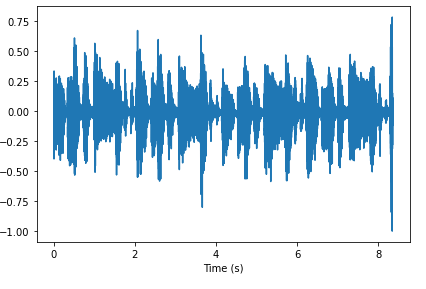
\includegraphics[scale=1]{fig/lab01/lab01_01.png}
		\caption{График всего звука}
	\end{center}
\end{figure}

Выделим полусекундный фрагмен, в котором высота постоянна и построим его график
\begin{lstlisting}[language=Python]
segment = wave.segment(start=5.2, duration=0.5)
segment.make_audio()

segment.plot()
decorate(xlabel='Time (s)')
\end{lstlisting}

\begin{figure}[H]
	\begin{center}
		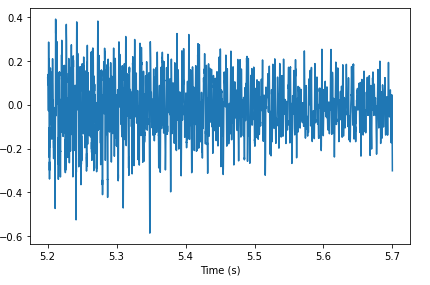
\includegraphics[scale=1]{fig/lab01/lab01_02.png}
		\caption{График сегмента звука}
	\end{center}
\end{figure}

Спектр сегмента
\begin{lstlisting}[language=Python]
spectrum = segment.make_spectrum()
spectrum.plot(high=5000)
decorate(xlabel='Frequency (Hz)')
\end{lstlisting}

\begin{figure}[H]
	\begin{center}
		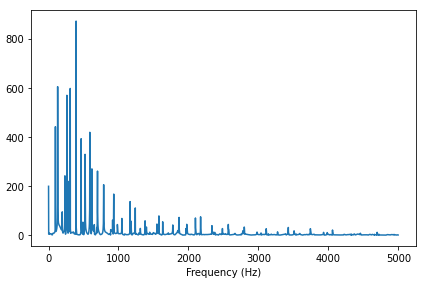
\includegraphics[scale=1]{fig/lab01/lab01_03.png}
		\caption{Спектр сегмента звука}
	\end{center}
\end{figure}

Осуществим фильтрацию при помощи специальных функций

Уберем частоты ниже 450
\begin{lstlisting}[language=Python]
spectrum.high_pass(450)
spectrum.plot(high=5000)
decorate(xlabel='Frequency (Hz)')
\end{lstlisting}

\begin{figure}[H]
	\begin{center}
		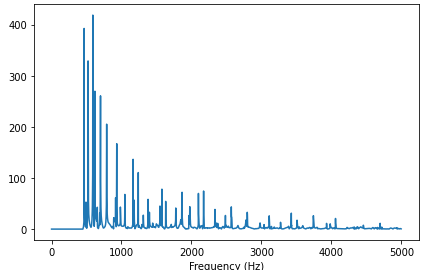
\includegraphics[scale=1]{fig/lab01/lab01_04.png}
		\caption{График частот без тех, что ниже 450}
	\end{center}
\end{figure}

Уберем частоты выше 2000
\begin{lstlisting}[language=Python]
spectrum.low_pass(2000)
spectrum.plot(high=5000)
decorate(xlabel='Frequency (Hz)')
\end{lstlisting}

\begin{figure}[H]
	\begin{center}
		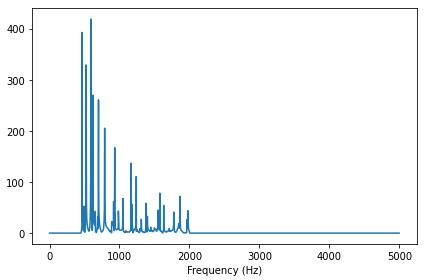
\includegraphics[scale=1]{fig/lab01/lab01_05.png}
		\caption{График частот без тех, что выше 2000}
	\end{center}
\end{figure}

Применим ФПЗ, чтобы убрать частоты в срезе
\begin{lstlisting}[language=Python]
spectrum.band_stop(500, 1100)
spectrum.plot(high=5000)
decorate(xlabel='Frequency (Hz)')
\end{lstlisting}

\begin{figure}[H]
	\begin{center}
		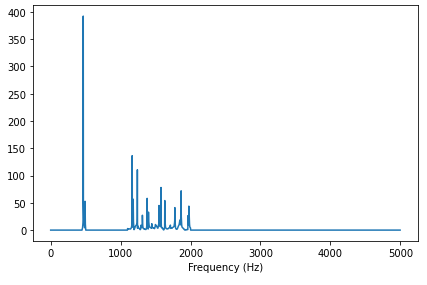
\includegraphics[scale=1]{fig/lab01/lab01_06.png}
		\caption{График частот после применения ФПЗ}
	\end{center}
\end{figure}

Преобразуем спектр обратно в сигнал
\begin{lstlisting}[language=Python]
test = spectrum.make_wave()
test.plot()
decorate(xlabel='Time (s)')
\end{lstlisting}

\begin{figure}[H]
	\begin{center}
		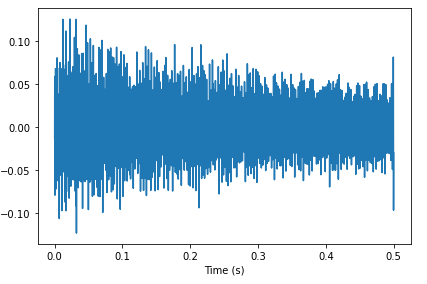
\includegraphics[scale=1]{fig/lab01/lab01_07.png}
		\caption{График преобразованного сигнала}
	\end{center}
\end{figure}

Проведем сравнение изначального среза и отфильтрованного

Изначальный:
\begin{lstlisting}[language=Python]
segment.make_audio()
\end{lstlisting}

Отфильтрованный:
\begin{lstlisting}[language=Python]
segment.make_audio()
\end{lstlisting}

Можно сделать вывод, что отфильрованный звук лишен объема (получился "плоский" звук)


\subsection{Упражнение 2}

Создайте сложный сигнал из объектов SinSignal и CosSignal, суммируя их. Обработайте сигнал для получения wave и прослушайте его. Вычислите Spectrum и распечатайте. Что произойдёт при добавлении частотных компонент, не кратных основным?

Создадим сложный сигнал из объектов SinSignal и CosSignal, суммируя их
\begin{lstlisting}[language=Python]
cos_sig = CosSignal(freq=300, amp=1.2, offset=0)
sin_sig = SinSignal(freq=100, amp=0.4, offset=0)
sin_sig2 = SinSignal(freq=700, amp=0.1, offset=0)
m_sig = cos_sig + sin_sig + sin_sig2
\end{lstlisting}

Построим график суммы
\begin{figure}[H]
	\begin{center}
		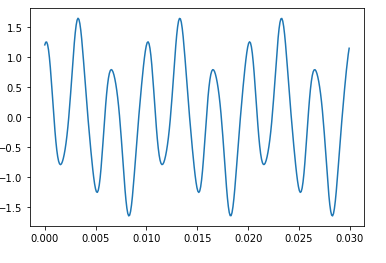
\includegraphics[scale=1]{fig/lab01/lab01_08.png}
		\caption{Графиксуммы сигналов}
	\end{center}
\end{figure}

Сделаем wave и послушаем
\begin{lstlisting}[language=Python]
wave = m_sig.make_wave()

wave.make_audio()
\end{lstlisting}

Вычислим спектр
\begin{lstlisting}[language=Python]
spectrum = wave.make_spectrum()
spectrum.plot()
\end{lstlisting}

\begin{figure}[H]
	\begin{center}
		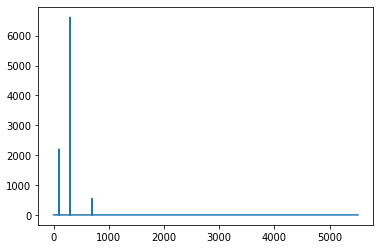
\includegraphics[scale=1]{fig/lab01/lab01_09.png}
		\caption{Спектр сигнала}
	\end{center}
\end{figure}

Теперь добавим частотный компонент, не кратный основным
\begin{lstlisting}[language=Python]
wave_2 = (m_sig + CosSignal(freq=550, amp=0.66, offset=0)).make_wave()
wave_2.make_audio()

wave_2.make_spectrum().plot()
\end{lstlisting}

\begin{figure}[H]
	\begin{center}
		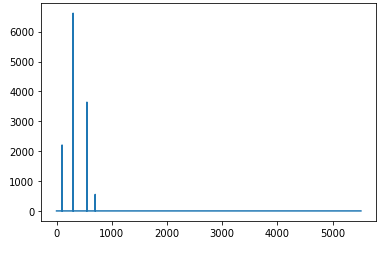
\includegraphics[scale=1]{fig/lab01/lab01_10.png}
		\caption{График после добавления частотного компонента}
	\end{center}
\end{figure}

Звук перестал быть однотонным


\subsection{Упражнение 3}

Напишите функцию strech, берущую wave и коэффицент изменения. Она должна ускорять или замедлять сигнал изменением ts и framerate.

Создадим функцию stretch, которая будет замедлять или ускорять сигнал в зависимости от коэффициента измнения
\begin{lstlisting}[language=Python]
def stretch(wave, coef):
  wave.ts *= coef
  wave.framerate /= coef
  
wave = read_wave('469283__matt141141__cm7-dm7-115bpm-loop.wav')
wave.make_audio()
\end{lstlisting}

Проверим замедление в 2 раза
\begin{lstlisting}[language=Python]
slow_wave = wave
stretch(slow_wave, 2)
slow_wave.make_audio()
\end{lstlisting}

Исходя из результатов видно, что звук замедлился в 2 раза, так как длинна дорожки в секундах, стала в 2 раза дольше

Проверим ускорение в 2 раза
\begin{lstlisting}[language=Python]
fast_wave = wave
stretch(fast_wave, 0.5)
fast_wave.make_audio()
\end{lstlisting}

Исходя из результатов видно, что звук ускорился в 2 раза, так как длинна дорожки в секундах, стала в 2 раза меньше


\subsection{Вывод}
В ходе данной работы было выполнено знакомство с основыми понятиями при работе со звуками и сигналами. При помощи библиотеки thinkDSP открывается множество возможностей по взаимодействию с сингалами, таких как их созданию, так и для их обработки
\newpage

\section{Гармоники}
\subsection{Упражнение 1}

Пилообразный сигнал линейно нарастает от -1 до 1, а затем резко падает до -1 и повторяется.

\noindent Напишите класс, называемый SawtoothSignal, расширяющий signal и предоставляющий evaluate для оценки пилообразного сигнала.

\noindent Вычислите спектр пилообразного сигнала. Как соотносится его гармоническая структура с тругольными с прямоугольными сигналами?

Создадим класс SawtoothSignal:

\begin{lstlisting}[language=Python]
import thinkdsp

class SawtoothSignal(thinkdsp.Sinusoid):
  def evaluate(self, ts):
    cycles = self.freq * ts + self.offset /np.pi / 2
    frac, _ = np.modf(cycles)
    ys = thinkdsp.normalize(thinkdsp.unbias(frac), self.amp)
    return ys
\end{lstlisting}

Построим график пилообразного сигнала:

\begin{lstlisting}[language=Python]
saw_signal = SawtoothSignal()
saw_signal.plot()
saw_wave = saw_signal.make_wave(duration=2, framerate=10000)
decorate(xlabel='Time (s)')
\end{lstlisting}

\begin{figure}[H]
	\begin{center}
		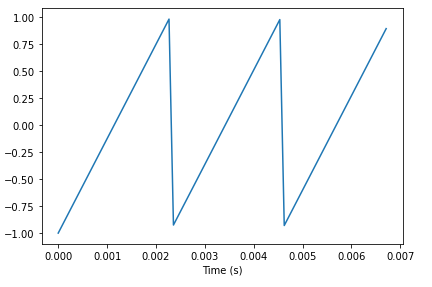
\includegraphics[scale=1]{fig/lab02/lab02_01.png}
		\caption{График пилообразного сигнала}
	\end{center}
\end{figure}

Вычислим спектр:

\begin{lstlisting}[language=Python]
spectr = saw_wave.make_spectrum()
spectr.plot()
decorate(xlabel='Frequency (Hz)')
\end{lstlisting}

\begin{figure}[H]
	\begin{center}
		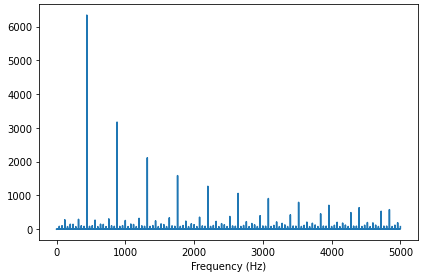
\includegraphics[scale=1]{fig/lab02/lab02_02.png}
		\caption{График спектра пилообразного сигнала}
	\end{center}
\end{figure}

Построим треугольный сигнал и вычислим его спектр:

\begin{lstlisting}[language=Python]
triangle_signal = TriangleSignal()
triangle_signal.plot()
decorate(xlabel='Time (s)')
\end{lstlisting}

\begin{figure}[H]
	\begin{center}
		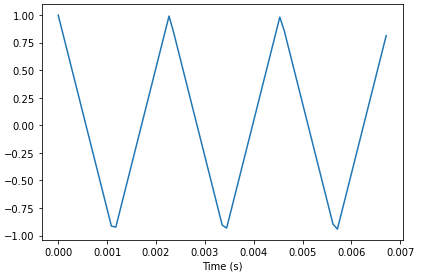
\includegraphics[scale=1]{fig/lab02/lab02_03.png}
		\caption{График треугольного сигнала}
	\end{center}
\end{figure}

\begin{lstlisting}[language=Python]
triangle_signal.make_wave(duration=2, framerate=10000).make_spectrum().plot()
decorate(xlabel='Frequency (Hz)')
\end{lstlisting}

\begin{figure}[H]
	\begin{center}
		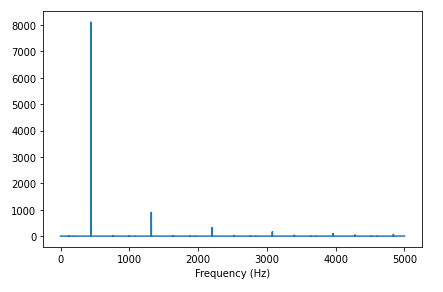
\includegraphics[scale=1]{fig/lab02/lab02_04.png}
		\caption{График спектра треугольного сигнала}
	\end{center}
\end{figure}

Построим прямоугольный сигнал и вычислим его спектр:

\begin{lstlisting}[language=Python]
square_signal = SquareSignal()
square_signal.plot()
decorate(xlabel='Time (s)')
\end{lstlisting}

\begin{figure}[H]
	\begin{center}
		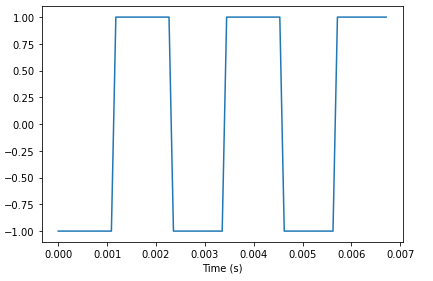
\includegraphics[scale=1]{fig/lab02/lab02_05.png}
		\caption{График прямоугольного сигнала}
	\end{center}
\end{figure}

\begin{lstlisting}[language=Python]
square_signal.make_wave(duration=2, framerate=10000).make_spectrum().plot()
decorate(xlabel='Frequency (Hz)')
\end{lstlisting}

\begin{figure}[H]
	\begin{center}
		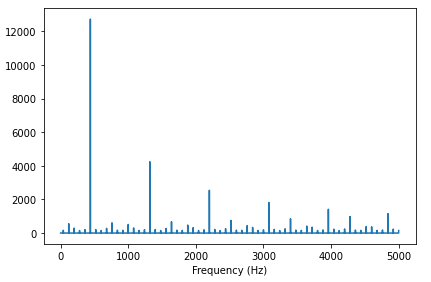
\includegraphics[scale=1]{fig/lab02/lab02_06.png}
		\caption{График спектра прямоугольного сигнала}
	\end{center}
\end{figure}

Если сравнивать гармоническую структуру пилообразного сигнала с треугольным сигналом, то у треугольного сигнала амплитуда будет падать пропорционально квадрату частоты, а у пилообразного - пропорционально частоте, также как и прямоугольного.

Если сравнивать гармоники, то у треугольного и прямоугольного сигналов есть только нечетные, а у пилообразного - четные и нечетные гармоники


\subsection{Упражнение 2}

Создайте прямугольный сигнал 1100 Гц и вычислите wave с выборками 10 000 кадров в секунду. Постройте спектр и убедитесь, что большинство гармоник "завёрнуты" из-за биений, слышно ли последствия этого при проигрывании?

Создадим квадртаный сигнал с частотой 1100 Hz и с выборкой кадров в секунду 10000

\begin{lstlisting}[language=Python]
square = SquareSignal(1100)
square_wave = square.make_wave(duration = 1, framerate=10000)
square_wave.make_spectrum().plot()
decorate(xlabel='Frequency (Hz)')
\end{lstlisting}

\begin{figure}[H]
	\begin{center}
		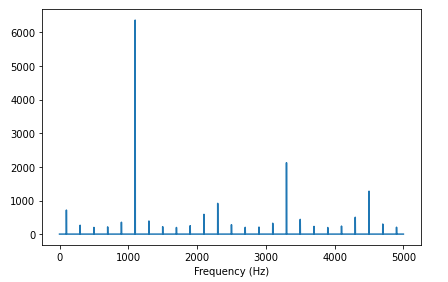
\includegraphics[scale=1]{fig/lab02/lab02_07.png}
		\caption{График прямоугольного сигнала с частотой 1100 Hz}
	\end{center}
\end{figure}

На спектре видна завернутость гармоник из-за биений
\begin{lstlisting}[language=Python]
square_wave.make_audio()
\end{lstlisting}


\subsection{Упражнение 3}

Возьмите объект спектра spectrum, и выведите первые несколько значений spectrum.fs, вы увидите, что частоты начинаются с нуля. Итак, «spectrum.hs[0]» — это величина компонента с частотой 0. Но что это значит?

\noindent Попробуйте этот эксперимент:

1. Сделать треугольный сигнал с частотой 440 и создать Волну длительностью 0,01 секунды. Постройте форму волны.

2. Создайте объект Spectrum и напечатайте spectrum.hs[0]. Каковы амплитуда и фаза этой составляющей?

3. Установите spectrum.hs[0] = 100. Создайте волну из модифицированного спектра и выведите ее. Как эта операция влияет на форму сигнала?

Создадим треугольный сигнал с частотой 440Hz и wave длительонстью 0,01 секунд

\begin{lstlisting}[language=Python]
triangle = TriangleSignal(440)
triangle_wave = triangle.make_wave(duration=0.01)
triangle_wave.plot()
decorate(xlabel='Time (s)')
\end{lstlisting}

\begin{figure}[H]
	\begin{center}
		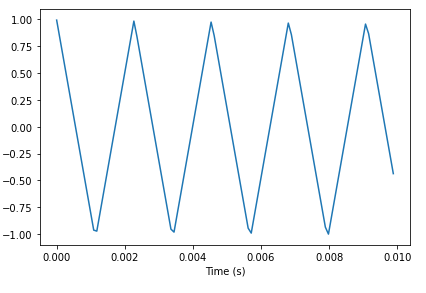
\includegraphics[scale=1]{fig/lab02/lab02_08.png}
		\caption{График треугольного сигнала с частотой 440 Hz}
	\end{center}
\end{figure}

Убедимся в том, что первый элемент массива hs объекта Spectrum - комплексное число, близкое к нулю

\begin{lstlisting}[language=Python]
tr_sp = triangle_wave.make_spectrum()
tr_sp.hs[0]

(1.0436096431476471e-14+0j)
\end{lstlisting}

Присвоим первому элементу значение 100 и построим график

\begin{lstlisting}[language=Python]
tr_sp.hs[0] = 100
tr_sp.make_wave().plot()
decorate(xlabel='Time (s)')
\end{lstlisting}

\begin{figure}[H]
	\begin{center}
		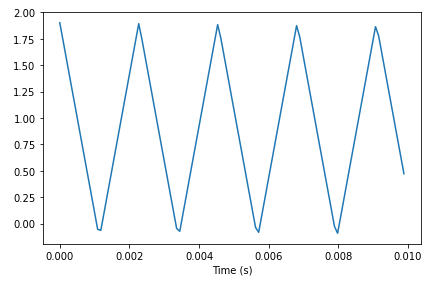
\includegraphics[scale=1]{fig/lab02/lab02_09.png}
		\caption{Обновленный график сигнала}
	\end{center}
\end{figure}

Исходя из графика можно сделать вывод, что сигнал сместился по вертикали. Значит первый элемент hs отвечает за смещение по вертикали и если он близок к нулю, то сигнал не смещается


\subsection{Упражнение 4}

Напишите функцию, которая принимает Spectrum в качестве параметра и модифицирует его, деля каждый элемент hs на соответствующую частоту из fs. Протестируйте свою функцию, используя один из файлов WAV в репозитории или любой объект Wave.

1. Рассчитайте спектр и начертите его.

2. Измените спектр, используя свою функцию, и снова начертите его.

3. Сделать волну из модифицированного Spectrum и прослушать ее. Как эта операция влияет на сигнал?

Создадим функцию, которая принимает на вход Spectrum и изменяет его делением каждого элемента hs на соответствующую частоту fs

\begin{lstlisting}[language=Python]
def spectrum_divide(sp):
  sp.hs[1:] /= sp.fs[1:]
  sp.hs[0] = 0
\end{lstlisting}

Проверим функцию на треугольном сигнале

\begin{lstlisting}[language=Python]
tr = TriangleSignal()
tr_wave = tr.make_wave(duration=0.5, framerate=10000)
tr_wave.make_audio()

tr_sp = tr_wave.make_spectrum()
tr_sp.plot()
decorate(xlabel='Frequency (Hz)')
\end{lstlisting}

\begin{figure}[H]
	\begin{center}
		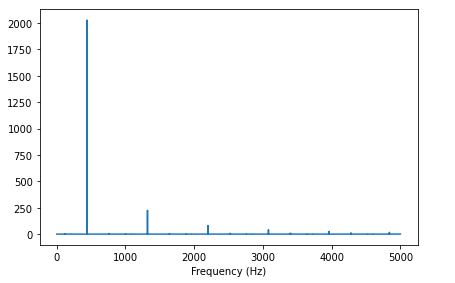
\includegraphics[scale=1]{fig/lab02/lab02_10.png}
		\caption{Спектр сигнала}
	\end{center}
\end{figure}

Применим функцию и посмотрим на результат

\begin{lstlisting}[language=Python]
spectrum_divide(tr_sp)
tr_sp.plot()
decorate(xlabel='Frequency (Hz)')
\end{lstlisting}

\begin{figure}[H]
	\begin{center}
		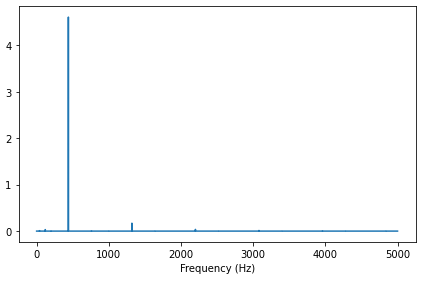
\includegraphics[scale=1]{fig/lab02/lab02_11.png}
		\caption{Спектр измененного сигнала}
	\end{center}
\end{figure}

\begin{lstlisting}[language=Python]
tr_sp.make_wave().make_audio()
\end{lstlisting}

Звук стал ниже, функция работает как ФНЧ


\subsection{Упражнение 5}

Треугольные и прямоугольные волны имеют только нечетные гармоники; пилообразная волна имеет как четные, так и нечетные гармоники. Гармоники прямоугольной и пилообразной волн затухают пропорционально $1/f$; гармоники треугольной волны затухают как $1/f^2$. Можете ли вы найти форму волны, в которой четные и нечетные гармоники затухают как $1/f^2$?

\noindent Подсказка: есть два способа подойти к этому: вы можете построить нужный сигнал путем сложения синусоид, или вы может начаться с сигнала, похожего на то, что вы хотите, и изменить его.

Создадим сигнал, который состоит из четных и нечетных гармоник, а также эти гармоники падают пропорционально квадрату частоты.

Возьмем пилообразный сигнал, который имет четные и нечетные гармоники, а далее скорректируем его спад при помощи функции из Упражения 2.5

\begin{lstlisting}[language=Python]
saw = SawtoothSignal(400)
saw_wave = saw.make_wave(duration=0.5, framerate=20000)
saw_sp = saw_wave.make_spectrum()
saw_sp.plot()
decorate(xlabel='Frequency (Hz)')
\end{lstlisting}

\begin{figure}[H]
	\begin{center}
		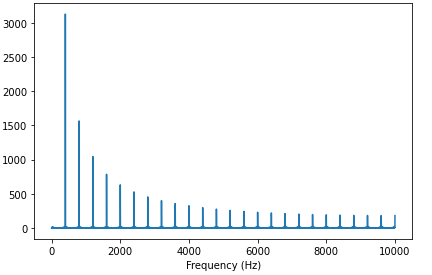
\includegraphics[scale=1]{fig/lab02/lab02_12.png}
		\caption{Спектр пилообразного сигнала}
	\end{center}
\end{figure}

Применим функцию для изменения амплитуды спада

\begin{lstlisting}[language=Python]
spectrum_divide(saw_sp)
saw_sp.scale(400)
saw_sp.plot()
decorate(xlabel='Frequency (Hz)')
\end{lstlisting}

\begin{figure}[H]
	\begin{center}
		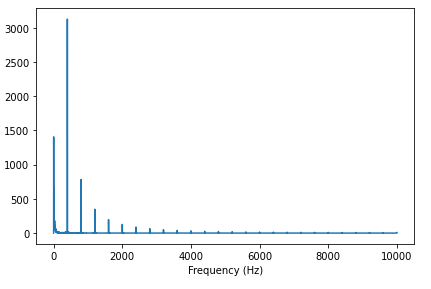
\includegraphics[scale=1]{fig/lab02/lab02_13.png}
		\caption{Спектр измененного сигнала}
	\end{center}
\end{figure}

Получается, что амплитуда падает пропорционально квадрату частоты, а также имеются четные и нечетные гармоники


\subsection{Вывод}

В данной работе были исследованы некоторые виды сигналов. Были рассмотрены спектры и гармонические структуры сигналов. Также в одном из пунктов были замечены биения и мы проверили их действие на звук.
\newpage

\section{Непериодические сигналы}
\subsection{Упражнение 1}

Запустите и прослушайте примеры в файле chap03.ipynb. В примере с утечкой попробуйте заменить окно Хэмминга одним из других окон, предоставляемых NumPy, и посмотрите, как они влияют на утечку.

Если длительность кратна периоду, то начало и конец отрезка совпадают, и мы получаем минимальную утечку.

\begin{lstlisting}[language=Python]
from thinkdsp import SinSignal

signal = SinSignal(freq=440)
duration = signal.period * 30
wave = signal.make_wave(duration)
wave.plot()
decorate(xlabel='Time (s)')

spectrum.plot(high=880)
\end{lstlisting}

\begin{figure}[H]
	\begin{center}
		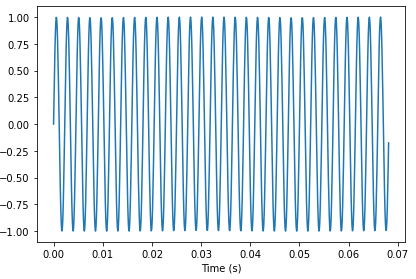
\includegraphics[scale=1]{fig/lab03/lab03_01.png}
		\caption{Рассматриваемый сигнал}
	\end{center}
\end{figure}

\begin{lstlisting}[language=Python]
spectrum = wave.make_spectrum()
spectrum.plot(high=880)
decorate(xlabel='Frequency (Hz)', ylabel='Amplitude')
\end{lstlisting}

\begin{figure}[H]
	\begin{center}
		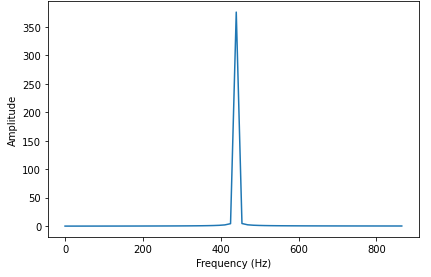
\includegraphics[scale=1]{fig/lab03/lab03_02.png}
		\caption{Спектр рассматриваемого сигнала}
	\end{center}
\end{figure}

Если продолжительность не кратна периоду, утечка довольно плохая.

\begin{lstlisting}[language=Python]
duration = signal.period * 30.25
wave = signal.make_wave(duration)
wave.plot()
decorate(xlabel='Time (s)')
\end{lstlisting}

\begin{figure}[H]
	\begin{center}
		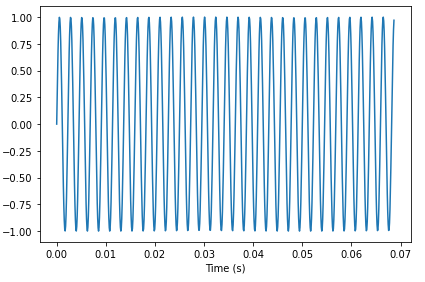
\includegraphics[scale=1]{fig/lab03/lab03_03.png}
		\caption{Рассматриваемый сигнал}
	\end{center}
\end{figure}

\begin{lstlisting}[language=Python]
spectrum = wave.make_spectrum()
spectrum.plot(high=880)
decorate(xlabel='Frequency (Hz)')
\end{lstlisting}

\begin{figure}[H]
	\begin{center}
		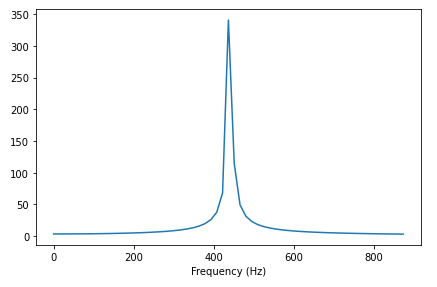
\includegraphics[scale=1]{fig/lab03/lab03_04.png}
		\caption{Спектр рассматриваемого сигнала}
	\end{center}
\end{figure}

Работа с окнами помогает (но обратите внимание, что она снижает общую энергию).

\begin{lstlisting}[language=Python]
wave.hamming()
spectrum = wave.make_spectrum()
spectrum.plot(high=880)
decorate(xlabel='Frequency (Hz)')
\end{lstlisting}

\begin{figure}[H]
	\begin{center}
		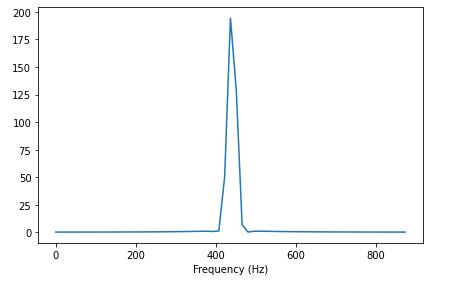
\includegraphics[scale=1]{fig/lab03/lab03_05.png}
		\caption{Спектр сигнала с применение окна Хээминга}
	\end{center}
\end{figure}

Если вы вслепую вычислите ДПФ непериодического сегмента, вы получите «размытие движения».

\begin{lstlisting}[language=Python]
signal = Chirp(start=220, end=440)
wave = signal.make_wave(duration=1)
spectrum = wave.make_spectrum()
spectrum.plot(high=700)
decorate(xlabel='Frequency (Hz)')
\end{lstlisting}

\begin{figure}[H]
	\begin{center}
		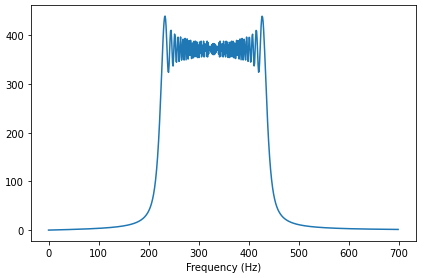
\includegraphics[scale=1]{fig/lab03/lab03_06.png}
		\caption{Спектр сигнала}
	\end{center}
\end{figure}

Спектрограмма — это визуализация кратковременного ДПФ, позволяющая увидеть, как спектр меняется во времени.

\begin{lstlisting}[language=Python]
def plot_spectrogram(wave, seg_length):
    """
    """
    spectrogram = wave.make_spectrogram(seg_length)
    print('Time resolution (s)', spectrogram.time_res)
    print('Frequency resolution (Hz)', spectrogram.freq_res)
    spectrogram.plot(high=700)
    decorate(xlabel='Time(s)', ylabel='Frequency (Hz)')
    
signal = Chirp(start=220, end=440)
wave = signal.make_wave(duration=1, framerate=11025)
plot_spectrogram(wave, 512)

Time resolution (s) 0.046439909297052155
Frequency resolution (Hz) 21.533203125
\end{lstlisting}

\begin{figure}[H]
	\begin{center}
		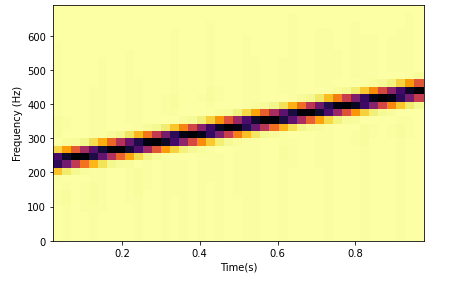
\includegraphics[scale=1]{fig/lab03/lab03_07.png}
		\caption{КПФ сигнала}
	\end{center}
\end{figure}

Если вы увеличите длину сегмента, вы получите лучшее разрешение по частоте, худшее разрешение по времени.

\begin{lstlisting}[language=Python]
plot_spectrogram(wave, 1024)

Time resolution (s) 0.09287981859410431
Frequency resolution (Hz) 10.7666015625
\end{lstlisting}

\begin{figure}[H]
	\begin{center}
		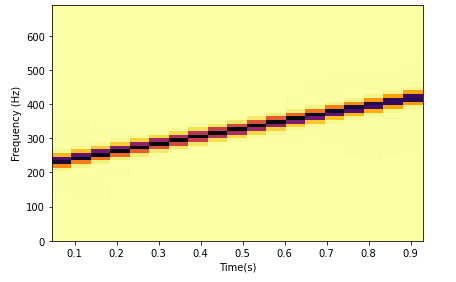
\includegraphics[scale=1]{fig/lab03/lab03_08.png}
		\caption{КПФ измененного сигнала}
	\end{center}
\end{figure}

Если вы уменьшите длину сегмента, вы получите лучшее временное разрешение, худшее разрешение по частоте.

\begin{lstlisting}[language=Python]
plot_spectrogram(wave, 256)

Time resolution (s) 0.023219954648526078
Frequency resolution (Hz) 43.06640625
\end{lstlisting}

\begin{figure}[H]
	\begin{center}
		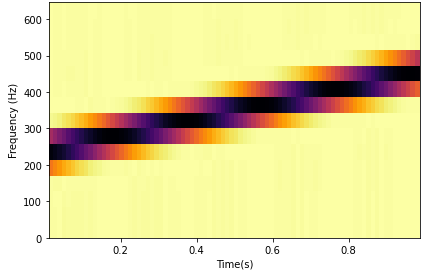
\includegraphics[scale=1]{fig/lab03/lab03_09.png}
		\caption{КПФ измененного сигнала}
	\end{center}
\end{figure}


\subsection{Упражнение 2}


Создадим класс SawtoothChirp, расширяющий Chirp и переопределяющий evaluate для генерации пилообразного сигнала с линейно увеличивающейся (или уменьшающейся) частотой

\begin{lstlisting}[language=Python]
from thinkdsp import Chirp
from thinkdsp import normalize, unbias

PI2 = 2 * np.pi

class SawtoothChirp(Chirp):

    def evaluate(self, ts):
        freqs = np.linspace(self.start, self.end, len(ts))
        dts = np.diff(ts, prepend=0)
        dphis = PI2 * freqs * dts
        phases = np.cumsum(dphis)
        cycles = phases / PI2
        frac, _ = np.modf(cycles)
        ys =  normalize(unbias(frac), self.amp)
        return ys
\end{lstlisting}

Протестируем полученный класс. Создадим пилообразный сигнал от 1318Hz до частоты 5274Hz

\begin{lstlisting}[language=Python]
sig = SawtoothChirp(1318, 5274)
w = sig.make_wave(duration = 4, framerate = 10000)
w.apodize()
w.make_audio()
\end{lstlisting}

Можно услышать биения

Теперь построим и распечатаем спектограмму этого сигнала

\begin{lstlisting}[language=Python]
sp = w.make_spectrogram(seg_length = 512)
sp.plot(high = 7000)
\end{lstlisting}

\begin{figure}[H]
	\begin{center}
		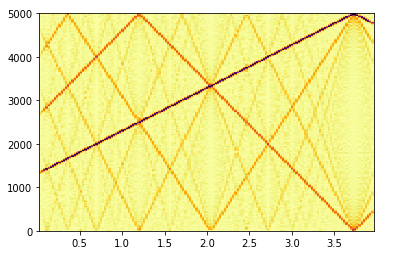
\includegraphics[scale=1]{fig/lab03/lab03_10.png}
		\caption{КПФ сигнала}
	\end{center}
\end{figure}


\subsection{Упражнение 3}

Создадим пилообразный чирп, меняющийся от 2500 до 3000 Гц, на его основе создадим сигнал длительностью 1 секунду и частотой кадров 20 кГц, рапечатаем его спектр

\begin{lstlisting}[language=Python]
signal = SawtoothChirp(start=2500, end=3000)
wave = signal.make_wave(duration=1, framerate=20000)
wave.make_audio()

wave.make_spectrum().plot()
decorate(xlabel='Frequency (Hz)')
\end{lstlisting}

\begin{figure}[H]
	\begin{center}
		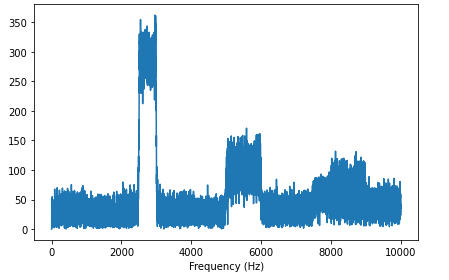
\includegraphics[scale=1]{fig/lab03/lab03_11.png}
		\caption{Спектр сигнала}
	\end{center}
\end{figure}

Из графика видно, что базовая частота колеблется от 2500 до 3000 Hz. Также видны следующие гармоники на частотах от 5000-6000 Hz и от 7500-9000 Hz

\subsection{Упражнение 4}

В музыкальной терминологии «глиссандо» — это нота, которая скользит от одной высоты тона к другой, поэтому она похожа на чириканье. Найдите или сделайте запись глиссандо и постройте его спектрограмму.

Найдем и распечатаем звук глиссандо и распечатаем спектограмму

\begin{lstlisting}[language=Python]
if not os.path.exists('495734__phonosupf__sax-glissando.wav'):
    !wget https://github.com/sergeyfedorov02/Telecom/raw/main/495734__phonosupf__sax-glissando.wav
    
from thinkdsp import read_wave

wave = read_wave('495734__phonosupf__sax-glissando.wav')
wave.make_audio()

wave.make_spectrogram(512).plot(high=5000)
decorate(xlabel='Time (s)', ylabel='Frequency (Hz)')
\end{lstlisting}

\begin{figure}[H]
	\begin{center}
		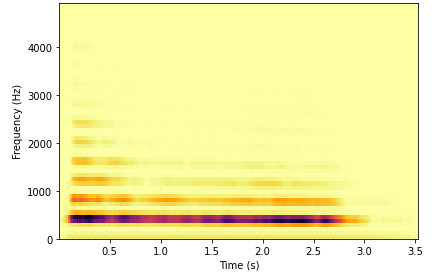
\includegraphics[scale=1]{fig/lab03/lab03_12.png}
		\caption{Спектрограмма сигнала}
	\end{center}
\end{figure}

Видим, что спектограмма очень похожа на наш чирп.

\subsection{Упражнение 5}

Тромбонист может играть глиссандо, выдвигая слайд тромбона и непрерывно дуя. По мере выдвижения ползуна общая длина трубки увеличивается, а результирующий шаг обратно пропорционален длине.
Предполагая, что игрок перемещает слайд с постоянной скоростью, как меняется ли частота со временем?

\noindent Напишите класс TromboneGliss, расширяющий класс Chirp и предоставляет evaluate. Создайте волну, имитирующую тромбон глиссандо от F3 вниз до C3 и обратно до F3. C3 — 262 Гц; F3 есть 349 Гц.

Напишем класс TromboneGliss расширяющий класс Chirp и переопределяющий метод evaluate. Для этого для вычисления частоты используется функция np.linspace, но в аргументы передается не просто начальная и конечная частоты, а единица деленная на эти частоты

\begin{lstlisting}[language=Python]
class TromboneGliss(Chirp):
        
    def evaluate(self, ts):
        l1, l2 = 1.0 / self.start, 1.0 / self.end
        lengths = np.linspace(l1, l2, len(ts))
        freqs = 1 / lengths
        
        dts = np.diff(ts, prepend=0)
        dphis = PI2 * freqs * dts
        phases = np.cumsum(dphis)
        ys = self.amp * np.cos(phases)
        return ys
\end{lstlisting}

Создадим два сигнала-глиссандо от C3 до F3 и обратно, воспроизведем эти звуки, своместим два сигнала в один и построим его спектограмму

\begin{lstlisting}[language=Python]
sig = TromboneGliss(262, 349)
w1 = sig.make_wave(duration=1)
w1.apodize()
w1.make_audio()

sig = TromboneGliss(349, 262)
w2 = sig.make_wave(duration=1)
w2.apodize()
w2.make_audio()

w = w1 | w2
w.make_audio()

sp = wave.make_spectrogram(1024)
sp.plot(high=1000)
decorate(xlabel='Time (s)', ylabel='Frequency (Hz)')
\end{lstlisting}

\begin{figure}[H]
	\begin{center}
		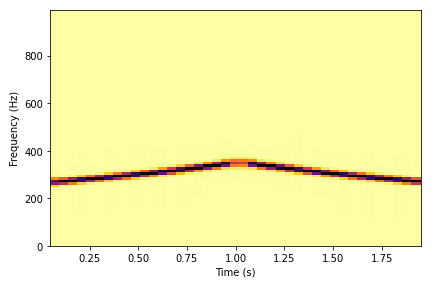
\includegraphics[scale=1]{fig/lab03/lab03_13.png}
		\caption{Спектрограмма сигнала}
	\end{center}
\end{figure}

Как видно из графика и звуков, частота сначала возрастает, а затем спадает до начальной


\subsection{Упражнение 6}

Найдем запись серии гласных звуков и посмотрим на спектограмму

\begin{lstlisting}[language=Python]
if not os.path.exists('code_87778__marcgascon7__vocals.wav'):
    !wget https://github.com/sergeyfedorov02/Telecom/raw/main/code_87778__marcgascon7__vocals.wav
    
wave = read_wave('code_87778__marcgascon7__vocals.wav')
wave.make_audio()

wave.make_spectrogram(1024).plot(high=1000)
decorate(xlabel='Time (s)', ylabel='Frequency (Hz)')
\end{lstlisting}

\begin{figure}[H]
	\begin{center}
		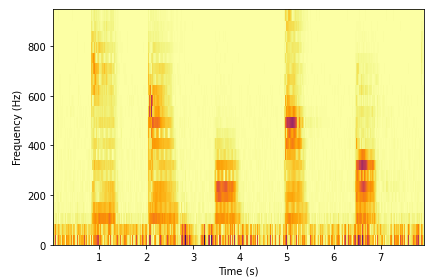
\includegraphics[scale=1]{fig/lab03/lab03_14.png}
		\caption{Спектрограмма гласных звуков}
	\end{center}
\end{figure}

Исходя из графика видно, что фоновый шум - это полоса снизу, а пики - это форманты. Также гласные звуки отличаются по соотношению амплитуд первых двух формант по отношению к основному

\begin{lstlisting}[language=Python]
seg = wave.segment(start=1, duration=0.25)
seg.make_spectrum().plot(high=1000)
decorate(xlabel='Frequency (Hz)')
\end{lstlisting}

\begin{figure}[H]
	\begin{center}
		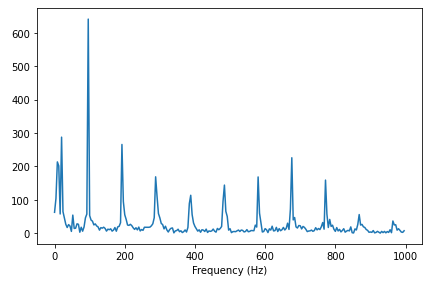
\includegraphics[scale=1]{fig/lab03/lab03_15.png}
		\caption{График частот для звука "ah"}
	\end{center}
\end{figure}

Исходя из графика видно, что основная частота равна 100 Hz, которая соответствует звуку "ah"

\begin{lstlisting}[language=Python]
seg = wave.segment(start=2.2, duration=0.25)
seg.make_spectrum().plot(high=1000)
decorate(xlabel='Frequency (Hz)')
\end{lstlisting}

\begin{figure}[H]
	\begin{center}
		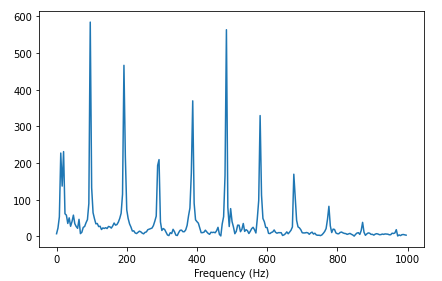
\includegraphics[scale=1]{fig/lab03/lab03_16.png}
		\caption{График частот для звука "eh"}
	\end{center}
\end{figure}

У звука "eh" высокоамплитудная форманта равна 500 Hz

\begin{lstlisting}[language=Python]
seg = wave.segment(start=3.5, duration=0.25)
seg.make_spectrum().plot(high=1000)
decorate(xlabel='Frequency (Hz)')
\end{lstlisting}

\begin{figure}[H]
	\begin{center}
		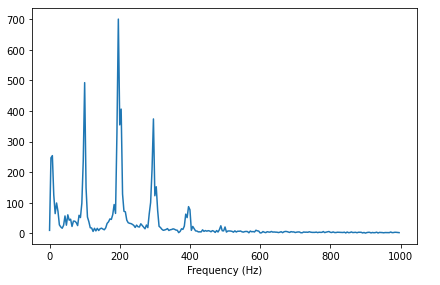
\includegraphics[scale=1]{fig/lab03/lab03_17.png}
		\caption{График частот для звука "ih"}
	\end{center}
\end{figure}

Видно, что у звука "ih" нет высокочастотных составляющих

\begin{lstlisting}[language=Python]
seg = wave.segment(start=5.1, duration=0.25)
seg.make_spectrum().plot(high=1000)
decorate(xlabel='Frequency (Hz)')
\end{lstlisting}

\begin{figure}[H]
	\begin{center}
		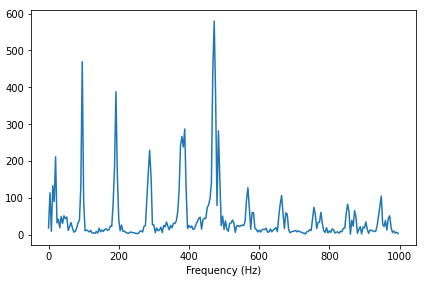
\includegraphics[scale=1]{fig/lab03/lab03_18.png}
		\caption{График частот для звука "oh"}
	\end{center}
\end{figure}

У звука "oh" высокоамплитудная форманта равна 500 Hz

\begin{lstlisting}[language=Python]
seg = wave.segment(start=6.5, duration=0.25)
seg.make_spectrum().plot(high=1000)
decorate(xlabel='Frequency (Hz)')
\end{lstlisting}

\begin{figure}[H]
	\begin{center}
		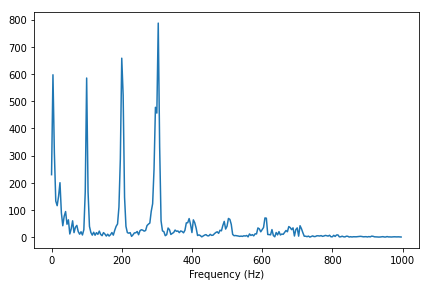
\includegraphics[scale=1]{fig/lab03/lab03_19.png}
		\caption{График частот для звука "oo"}
	\end{center}
\end{figure}

У звука "oo" высокоамплитудная форманта равна 300 Hz


\subsection{Вывод}

В этой работе были расмотрены апериодические сигналы, частотные компоненты которых изменяются во времени. Также в этой главе были рассмотрены спектрограммы - способ визуализации апериодичных сигналов.

\newpage

\section{Шумы}
\subsection{Упражнение 1}

«A Soft Murmur» — это веб-сайт, на котором можно послушать множество естественных источников шума, включая дождь, волны, ветер и т. д. 

\noindent На http://asoftmurmur.com/about/ вы можете найти их список записей, большинство из которых находится на http://freesound.org.

\noindent Загрузите несколько таких файлов и вычислите спектр каждого сигнала. Спектр мощности похож на белый шум, розовый шум, или броуновский шум? Как изменяется спектр во времени?

Возьмем два звука: пение птиц и дождь. Выделим из этих звуков короткие сегменты и построим спектры полученных сигналов.

\begin{lstlisting}[language=Python]
if not os.path.exists('28239__herbertboland__forestbirds.wav'):
    !wget https://github.com/sergeyfedorov02/Telecom/raw/main/28239__herbertboland__forestbirds.wav
    
from thinkdsp import read_wave

wave_birdsong = read_wave('28239__herbertboland__forestbirds.wav')
wave_birdsong = wave_birdsong.segment(start = 0, duration = 6)
wave_birdsong.make_audio()

spec = wave_birdsong.make_spectrum()
spec.plot_power(high = 200)
decorate(xlabel='Frequency (Hz)', ylabel='Power')
\end{lstlisting}

\begin{figure}[H]
	\begin{center}
		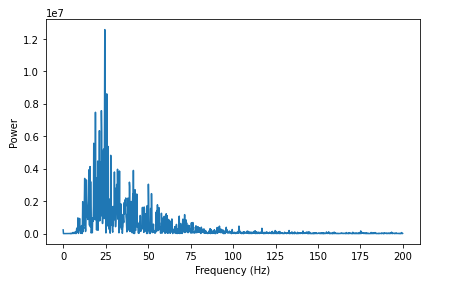
\includegraphics[scale=1]{fig/lab04/lab04_01.png}
		\caption{График сигнала}
	\end{center}
\end{figure}

Исходя из графика видно, что зависимость падения амплитуды от частоты напоминает розовый и бкелый шум (линейная зависимость). Посмотрим на спектр мощности в лагорифмическом масштабе.

\begin{lstlisting}[language=Python]
spec.plot_power()
log_birdsong = dict(xscale='log', yscale='log')
decorate(xlabel='Frequency (Hz)', ylabel='Power', **log_birdsong)
\end{lstlisting}

\begin{figure}[H]
	\begin{center}
		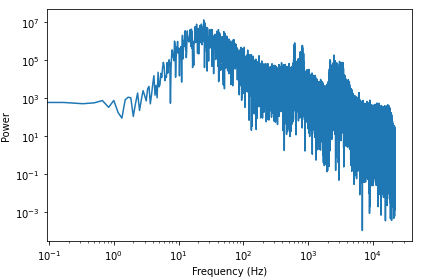
\includegraphics[scale=1]{fig/lab04/lab04_02.png}
		\caption{Спектр в логорифмическом масштабе}
	\end{center}
\end{figure}

Значение сначала возрастает, а потом уменьшается (падение удет линейно).

Рассмотрим следующий сигнал:

\begin{lstlisting}[language=Python]
if not os.path.exists('346641__inspectorj__rain-on-windows-interior-b.wav'):
    !wget https://github.com/sergeyfedorov02/Telecom/raw/main/346641__inspectorj__rain-on-windows-interior-b.wav
    
wave_rain = read_wave('346641__inspectorj__rain-on-windows-interior-b.wav')
wave_rain = wave_rain.segment(start = 0, duration = 6)
wave_rain.make_audio()

spec = wave_rain.make_spectrum()
spec.plot_power(high = 200)
decorate(xlabel='Frequency (Hz)', ylabel='Power')
\end{lstlisting}

\begin{figure}[H]
	\begin{center}
		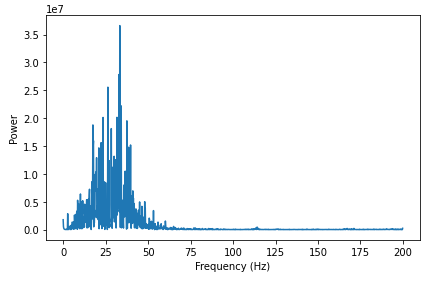
\includegraphics[scale=1]{fig/lab04/lab04_03.png}
		\caption{График сигнала}
	\end{center}
\end{figure}

Данный график также похож на предыдущий, но зависимость падения более похожа на линейную. Построим график в лагорифмическом масштабе.

\begin{lstlisting}[language=Python]
spec.plot_power()
log_rain = dict(xscale='log', yscale='log')
decorate(xlabel='Frequency (Hz)', ylabel='Power', **log_rain)
\end{lstlisting}

\begin{figure}[H]
	\begin{center}
		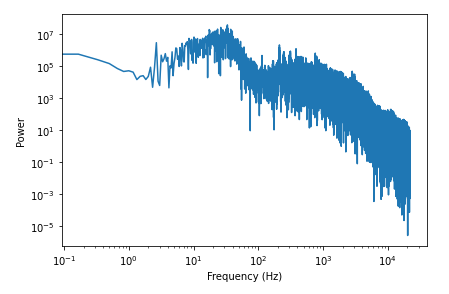
\includegraphics[scale=1]{fig/lab04/lab04_04.png}
		\caption{Спектр в логорифмическом масштабе}
	\end{center}
\end{figure}


\subsection{Упражнение 2}

Создадим метод barlet_method \cite{barlett}, который будет брать сигнал, разделять его на сегменты и вычислять спектр мощности для каждого сегмента и находить среднее по сегментам. Для этого нужно в аргументы функции сам сигнал и желаемую длину каждого сегмента. Затем вычислить спектр sp и выделить из него отдельные спектры specs. Потом выделить массив psds мощностей из каждого полученного спектра. Также вычислим среднюю мощность hs начального сигнала

\begin{lstlisting}[language=Python]
from thinkdsp import Spectrum

def barlet_method(wave, seg_length = 512, win_flag = True):
    sp = wave.make_spectrogram(seg_length, win_flag)
    specs = sp.spec_map.values()

    psds = [spectrum.power for spectrum in specs]
    hs = np.sqrt(sum(psds) / len(psds))
    fs = next(iter(specs)).fs

    return Spectrum(hs, fs, wave.framerate)
\end{lstlisting}

Проверим работоспособность функции на звуках из Упражнение 4.1

\begin{lstlisting}[language=Python]
psd = barlet_method(wave_birdsong)
psd.plot_power()
log_test_1 = dict(xscale='log', yscale='log')
decorate(xlabel='Frequency (Hz)', ylabel='Power', **log_test_1)
\end{lstlisting}

\begin{figure}[H]
	\begin{center}
		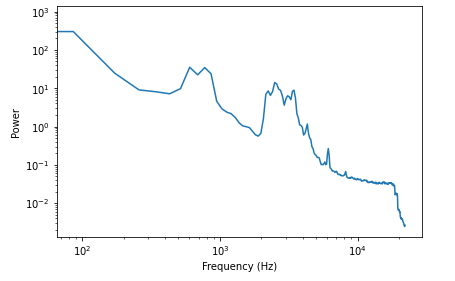
\includegraphics[scale=1]{fig/lab04/lab04_05.png}
		\caption{Результаты применения функции к первому сигналу из 4.1}
	\end{center}
\end{figure}

\begin{lstlisting}[language=Python]
psd = barlet_method(wave_rain)
psd.plot_power()
log_test_2 = dict(xscale='log', yscale='log')
decorate(xlabel='Frequency (Hz)', ylabel='Power', **log_test_2)
\end{lstlisting}

\begin{figure}[H]
	\begin{center}
		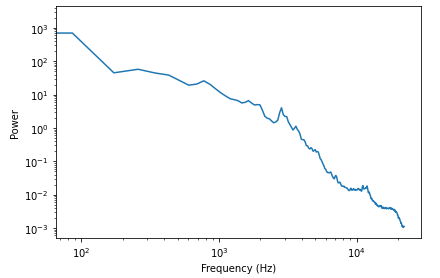
\includegraphics[scale=1]{fig/lab04/lab04_06.png}
		\caption{Результаты применения функции ко второму сигналу из 4.1}
	\end{center}
\end{figure}

Теперь зависимость между Частотой и Мощностью видна лучше, так во втором примере завимость больше похожа на линейную, как и говорилось ранее.


\subsection{Упражнение 3}

Откроем файл BTC.csv, который содержит исторические данные о ежедневной цене биткоина за последние полгода. Далее вычислим спектр цен как функцию от времени.

\begin{lstlisting}[language=Python]
if not os.path.exists('BTC_USD_2013-10-01_2020-03-26-CoinDesk.csv'):
    !wget https://github.com/AllenDowney/ThinkDSP/raw/master/code/BTC_USD_2013-10-01_2020-03-26-CoinDesk.csv
    
import pandas as pd

df = pd.read_csv('BTC_USD_2013-10-01_2020-03-26-CoinDesk.csv', parse_dates=[0])
df
\end{lstlisting}

\begin{figure}[H]
	\begin{center}
		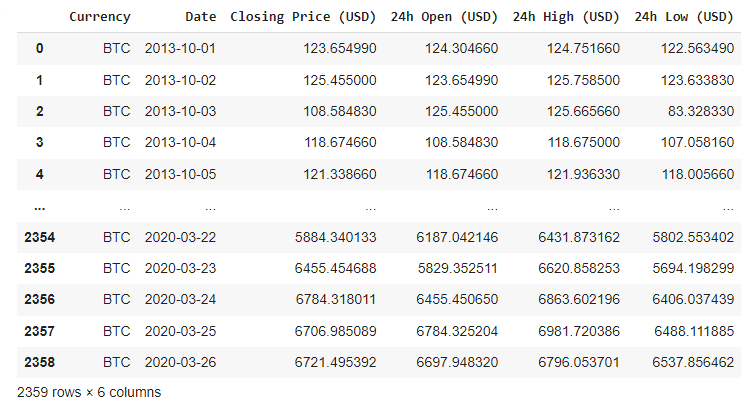
\includegraphics[scale=1]{fig/lab04/lab04_07.png}
		\caption{Таблица значений}
	\end{center}
\end{figure}

\begin{lstlisting}[language=Python]
ys = df['Closing Price (USD)']
ts = df.index

wave = thinkdsp.Wave(ys, ts, framerate = 1)
wave.plot()
decorate(xlabel='Дни')
\end{lstlisting}

\begin{figure}[H]
	\begin{center}
		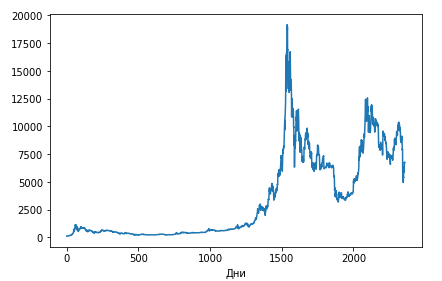
\includegraphics[scale=1]{fig/lab04/lab04_08.png}
		\caption{График цен BitCoin}
	\end{center}
\end{figure}

\begin{lstlisting}[language=Python]
spec = wave.make_spectrum()
spec.plot_power()
loglog = dict(xscale='log', yscale='log')
decorate(xlabel='Frequency (1/days)',
         ylabel='Power', 
         **loglog)
\end{lstlisting}

\begin{figure}[H]
	\begin{center}
		\includegraphics[scale=1]{fig/lab04/lab04_09.png}
		\caption{Спектрограмма цен BitCoin в логорифмическом формате}
	\end{center}
\end{figure}

\begin{lstlisting}[language=Python]
spec.estimate_slope()[0]

-1.7986681316517856
\end{lstlisting}

Красный шум должен иметь наклон -2. Наклон этой PSD близок к 1,7, поэтому трудно сказать, что это красным шумом или же разновидность розового шума.


\subsection{Упражнение 4}

Счетчик Гейгера — это прибор, который регистрирует радиацию. Когда ионизирующая частица попадает на детектор, он генерирует всплеск тока. Общий вывод в определенный момент времени можно смоделировать как некоррелированный шум Пуассона (UP), где каждая выборка представляет собой случайную величину из распределения Пуассона, которая соответствует количеству частиц, обнаруженных в течение интервала.

Напишем класс UncorrelatedPoissonNoise, который наследуется от класса thinkdsp._Noise, который моделирует некоррелированный пуассонвский шум (UP). Для этого следует переопределить функцию evaluate, в которой используется метод np.random.poisson(). Параметр этой функции lam - это среднее число частиц за время каждого интервала.

\begin{lstlisting}[language=Python]
from thinkdsp import Noise

class UncorrelatedPoissonNoise(Noise):
    def evaluate(self, ts):
      ys = np.random.poisson(self.amp, len(ts))
      return ys
\end{lstlisting}

Теперь сгенерируем сигнал с маленькой амплитудой(0.001) на основе этого класса. Ожидается услышать звук, как у счетчика Гейгера

\begin{lstlisting}[language=Python]
signal = UncorrelatedPoissonNoise(amp = 0.001)
wave = signal.make_wave(duration = 2, framerate = 10000)
wave.make_audio()

spec = wave.make_spectrum()
spec.plot_power()
decorate(xlabel='Frequency (Hz)', ylabel='Power', **loglog)
\end{lstlisting}

\begin{figure}[H]
	\begin{center}
		\includegraphics[scale=1]{fig/lab04/lab04_10.png}
		\caption{Получившийся спектр сигнала}
	\end{center}
\end{figure}

Теперь создадим такой же сигнал, но с большей амплитудой

\begin{lstlisting}[language=Python]
signal = UncorrelatedPoissonNoise(amp = 2)
wave = signal.make_wave(duration = 2, framerate = 10000)
wave.make_audio()

spec = wave.make_spectrum()
spec.plot_power()
decorate(xlabel='Frequency (Hz)', ylabel='Power', **loglog)
\end{lstlisting}

\begin{figure}[H]
	\begin{center}
		\includegraphics[scale=1]{fig/lab04/lab04_11.png}
		\caption{Получившийся спектр сигнала}
	\end{center}
\end{figure}

Результат стал похож на белый шум


\subsection{Упражнение 5}

В этой главе описан алгоритм генерации розового шума. Концептуально простой, но вычислительно затратный. Есть более эффективные альтернативы, такие как алгоритм Восса-Маккартни.

\noindent Исследуйте этот метод, реализуйте его, вычислите спектр и подтвердите, что он имеет желаемое отношение между мощностью и частотой.

Создадим функцию voss, которая реализаует более эффективный алгоритм Voss-McCartney для генерации розового шума. Вычислим спектр результата и убедимся в соответствии сотношения между мощностью и частотой.

\begin{lstlisting}[language=Python]
def voss(nrows, ncols=16):

    array = np.empty((nrows, ncols))
    array.fill(np.nan)
    array[0, :] = np.random.random(ncols)
    array[:, 0] = np.random.random(nrows)
    
    # Общее количество изменений равно nrows
    n = nrows
    cols = np.random.geometric(0.5, n)
    cols[cols >= ncols] = 0
    rows = np.random.randint(nrows, size=n)
    array[rows, cols] = np.random.random(n)

    df = pd.DataFrame(array)
    df.fillna(method='ffill', axis=0, inplace=True)
    total = df.sum(axis=1)

    return total.values
\end{lstlisting}

Проведем тестирование, для этого сгенерируем 10000 значений и превратим их в волну (построим график)

\begin{lstlisting}[language=Python]
ys = voss(10000)
ys

array([8.05587101, 6.94436007, 6.57274844, ..., 7.95820399, 8.83511144,
       8.77457504])
       
wave = thinkdsp.Wave(ys)
wave.unbias()
wave.normalize()
wave.plot()
\end{lstlisting}

\begin{figure}[H]
	\begin{center}
		\includegraphics[scale=1]{fig/lab04/lab04_12.png}
		\caption{Сгенерированный сигнал}
	\end{center}
\end{figure}

Получился случайный звук (шум), который меньше похож на белый шум, но выглядит более случайным, чем красный шум.

Прослушаем его:

\begin{lstlisting}[language=Python]
wave.make_audio()
\end{lstlisting}

Вычислим счпектр и наклон

\begin{lstlisting}[language=Python]
spec = wave.make_spectrum()
spec.hs[0] = 0
spec.plot_power()
decorate(xlabel='Frequency (Hz)',ylabel='Power',**loglog)
\end{lstlisting}

\begin{figure}[H]
	\begin{center}
		\includegraphics[scale=1]{fig/lab04/lab04_13.png}
		\caption{Спектр полученного шума}
	\end{center}
\end{figure}

\begin{lstlisting}[language=Python]
spec.estimate_slope().slope

-0.9928113664986493
\end{lstlisting}

Расчетный наклон близок к -1

Для более точной оценки сгенерируем более длинную выборку и воспользуемся методом Барлетта для вычисления среднего (найдем спектр средней мощности)

\begin{lstlisting}[language=Python]
import random

first = random.randint(50000, 70000)
first
69939

second = random.randint(100, 200)
second
129

wave = thinkdsp.Wave(voss(first * second))
spec = barlet_method(wave, seg_length=first, win_flag=False)
spec.hs[0] = 0
len(spec)
34970
\end{lstlisting}

Построим график

\begin{lstlisting}[language=Python]
spec.plot_power()
decorate(xlabel='Frequency (Hz)', ylabel='Power', **loglog)
\end{lstlisting}

\begin{figure}[H]
	\begin{center}
		\includegraphics[scale=1]{fig/lab04/lab04_14.png}
		\caption{Спектр средней мощности шума}
	\end{center}
\end{figure}

Данный график больше похож на прямую линию, лишь с некоторой кривизной на самых высоких частотах


\begin{lstlisting}[language=Python]
spec.estimate_slope().slope

-1.0014296136950736
\end{lstlisting}

Наклон стал ближе к -1


\subsection{Вывод}

В этой работе был рассмотрен шум. Шум - сигнал, содержащий компоненты с самыми разными частотами, но не имеющий гармонической структуры периодических сигналов, рассмотреных в предыдущих работах.
\newpage

\section{Автокорреляция }
\subsection{Упражнение 1}

Оцените высоты тона вокального чирпа для нескольких времён начала сегмента. Возьмем звук сирены

\begin{lstlisting}[language=Python]
if not os.path.exists('bcjordan__voicedownbew.wav'):
    !wget https://github.com/sergeyfedorov02/Telecom/raw/main/bcjordan__voicedownbew.wav

wave = read_wave('bcjordan__voicedownbew.wav')

wave.normalize()
wave.make_audio()

duration = 0.01
segment1 = wave.segment(start=0.1, duration=duration)
segment1.plot()
segment2 = wave.segment(start=0.2, duration=duration)
segment2.plot()
segment3 = wave.segment(start=0.3, duration=duration)
segment3.plot()
\end{lstlisting}

\begin{figure}[H]
	\begin{center}
		\includegraphics[scale=1]{fig/lab05/lab05_01.png}
		\caption{График выбранных сегментов}
	\end{center}
\end{figure}

Теперь воспользуемся автокорреляцией для определения высоты тона

\begin{lstlisting}[language=Python]
lags1, corrs1 = autocorr(segment1)
plt.plot(lags1, corrs1, color='green')
decorate(xlabel='Lag (index)', ylabel='Correlation', ylim=[-1, 1])

lags2, corrs2 = autocorr(segment2)
plt.plot(lags2, corrs2)
decorate(xlabel='Lag (index)', ylabel='Correlation', ylim=[-1, 1])

lags3, corrs3 = autocorr(segment3)
plt.plot(lags3, corrs3, color='red')
decorate(xlabel='Lag (index)', ylabel='Correlation', ylim=[-1, 1])
\end{lstlisting}

\begin{figure}[H]
	\begin{center}
		\includegraphics[scale=1]{fig/lab05/lab05_02.png}
		\caption{Автокорреляция сигналов}
	\end{center}
\end{figure}

Вычислим значения lags

\begin{lstlisting}[language=Python]
low, high = 50, 200
lag1 = np.array(corrs1[low:high]).argmax() + low

low, high = 50, 200
lag2 = np.array(corrs2[low:high]).argmax() + low

low, high = 50, 200
lag3 = np.array(corrs3[low:high]).argmax() + low

lag1, lag2, lag3

(91, 101, 109)
\end{lstlisting}

Вычислим периоды

\begin{lstlisting}
period1 = lag1 / segment1.framerate
period2 = lag2 / segment2.framerate
period3 = lag3 / segment3.framerate
period1, period2, period3

(0.0020634920634920637, 0.002290249433106576, 0.002471655328798186)
\end{lstlisting}

Теперь найдем F max

\begin{lstlisting}[language=Python]
frequency1 = 1 / period1
frequency2 = 1 / period2
frequency3 = 1 / period3
frequency1, frequency2, frequency3

(484.6153846153846, 436.63366336633663, 404.5871559633028)
\end{lstlisting}


\subsection{Упражнение 2}
Пример кода в chap05.ipynb показывает, как использовать автокорреляцию для оценки основной частоты периодического сигнала. Инкапсулируйте этот код в функцию estimate_dundamental, и используйте ее для отслеживания высоты тона записанного звука. Для тестирования возьмем тот же звук сирены

\begin{lstlisting}[language=Python]
wave.make_audio()
\end{lstlisting}

Построим спектограмму

\begin{lstlisting}[language=Python]
wave.make_spectrogram(2048).plot(high = 4200)
\end{lstlisting}

\begin{figure}[H]
	\begin{center}
		\includegraphics[scale=1]{fig/lab05/lab05_03.png}
		\caption{Спектрограмма записи}
	\end{center}
\end{figure}

Используем функцию estimate_fundamental из главы 5. Самый высокий пик в функции автокорреляции был отслежен с помощью выставления диапазона дагов для поиска от 70 до 200

\begin{lstlisting}[language=Python]
def estimate_fundamental(segment, low=70, high=200):
    lags, corrs = autocorr(segment)
    lag = np.array(corrs[low:high]).argmax() + low
    period = lag / segment.framerate
    frequency = 1 / period
    return frequency
    
duration = 0.01
segment = wave.segment(start=0.2, duration=duration)
freq = estimate_fundamental(segment)
freq

436.63366336633663
\end{lstlisting}

В цикле отследим пик по всему звуку. ts - это середина каждого сегмента

\begin{lstlisting}[language=Python]
step = 0.05
starts = np.arange(0.0, 1.4, step)

ts = []
freqs = []

for start in starts:
    ts.append(start + step/2)
    segment = wave.segment(start=start, duration=duration)
    freq = estimate_fundamental(segment)
    freqs.append(freq)
\end{lstlisting}

Синяя линия на графике наложена на спектограмму и показывает отслеживание высоты тона

\begin{lstlisting}[language=Python]
wave.make_spectrogram(2048).plot(high = 900)
plt.plot(ts, freqs, color='blue')
decorate(xlabel='Time (s)', ylabel='Frequency (Hz)')
\end{lstlisting}

\begin{figure}[H]
	\begin{center}
		\includegraphics[scale=1]{fig/lab05/lab05_04.png}
		\caption{Результат}
	\end{center}
\end{figure}


\subsection{Упражнение 3}

Возьмем данные о BitCoin из прошлой лабораторной работы и вычислим для этих данных автокорреляцию цен

\begin{lstlisting}[language=Python]
if not os.path.exists('BTC_USD_2013-10-01_2020-03-26-CoinDesk.csv'):
    !wget https://github.com/AllenDowney/ThinkDSP/raw/master/code/BTC_USD_2013-10-01_2020-03-26-CoinDesk.csv
    
import pandas as pd

df = pd.read_csv('BTC_USD_2013-10-01_2020-03-26-CoinDesk.csv', parse_dates=[0])
df

\end{lstlisting}

\begin{figure}[H]
	\begin{center}
		\includegraphics[scale=1]{fig/lab05/lab05_05.png}
		\caption{Таблица цены на BitCoin}
	\end{center}
\end{figure}

Вычислим автокорреляцию:

\begin{lstlisting}[language=Python]
ys = df['Closing Price (USD)']
ts = df.index

wave = Wave(ys, ts, framerate = 1)
wave.plot()
decorate(xlabel='Дни')
\end{lstlisting}

\begin{figure}[H]
	\begin{center}
		\includegraphics[scale=1]{fig/lab05/lab05_06.png}
		\caption{График цен на BitCoin}
	\end{center}
\end{figure}

\begin{lstlisting}[language=Python]
lags, corrs = autocorr(wave)
plt.plot(lags, corrs)
\end{lstlisting}

\begin{figure}[H]
	\begin{center}
		\includegraphics[scale=1]{fig/lab05/lab05_07.png}
		\caption{Автокорреляция функции цены на BitCoin}
	\end{center}
\end{figure}

Исходя из графика видно, что он постепенно снижается и похож на розовый шум. Также присутствует умеренная корреляция на 550 дне и 820. Теперь вычислим корреляцию на основе функции np.correlate, она не смещает и нормализует волну.

\begin{lstlisting}[language=Python]
corrs2 = np.correlate(wave.ys, wave.ys, mode = 'same')
lags = np.arange(-len(wave) // 2, len(wave) // 2)
plt.plot(lags, corrs2)
\end{lstlisting}

\begin{figure}[H]
	\begin{center}
		\includegraphics[scale=1]{fig/lab05/lab05_08.png}
		\caption{Автокорреляция функции цены на BitCoin при помощи np.correlate}
	\end{center}
\end{figure}

Вторая часть результатов (правая) соответствует положительными интервалам lags

\begin{lstlisting}[language=Python]
N = len(corrs2)
half = corrs[N//4:]
plt.plot(half)
\end{lstlisting}

\begin{figure}[H]
	\begin{center}
		\includegraphics[scale=1]{fig/lab05/lab05_09.png}
		\caption{Правая часть результатов}
	\end{center}
\end{figure}


\subsection{Упражнение 4}

В репозитории Jupyter есть блокнот saxophone.inypb, в котором исследуется автокорреляция, восприятие высоты тона и явление, называемое подавленная основная. Прочтите этот блокнто и "погоняйте" примеры. Выберите другой сегмент записи и вновь поработайте с примерами

\begin{lstlisting}[language=Python]
if not os.path.exists('100475__iluppai__saxophone-weep.wav'):
    !wget https://github.com/AllenDowney/ThinkDSP/raw/master/code/100475__iluppai__saxophone-weep.wav
    
wave = read_wave('100475__iluppai__saxophone-weep.wav')
wave.normalize()
wave.make_audio()
\end{lstlisting}

Построим спектограмму

\begin{lstlisting}[language=Python]
wave.make_spectrogram(1024).plot(high = 3000)
decorate(xlabel='Time (s)', ylabel='Frequency (Hz)')
\end{lstlisting}

\begin{figure}[H]
	\begin{center}
		\includegraphics[scale=1]{fig/lab05/lab05_10.png}
		\caption{Спектрограмма звука}
	\end{center}
\end{figure}

На графике видна гармоническая структура во времени

Теперь возьмем некоторый сегмент и "прогоним" его через функции из блокнота

\begin{lstlisting}[language=Python]
segment = wave.segment(start=1, duration=0.2)
segment.make_audio()

spectrum = segment.make_spectrum()
spectrum.plot(high=4000)
decorate(xlabel='Frequency (Hz)', ylabel='Amplitude')
\end{lstlisting}

\begin{figure}[H]
	\begin{center}
		\includegraphics[scale=1]{fig/lab05/lab05_11.png}
		\caption{Спектр звука}
	\end{center}
\end{figure}

Данный спектр похож на спектр квадратного сигнала. Пики находятся на 1245, 415 и 830 Гц

\begin{lstlisting}[language=Python]
spectrum.peaks()[:10]

[(1956.703292712428, 1245.0),
 (1034.570299739157, 415.0),
 (481.52480153206335, 830.0),
 (351.0776583833776, 2075.0),
 (275.4196733573752, 1250.0),
 (264.72288947314, 1240.0),
 (200.51232139688983, 2490.0),
 (188.9737445345148, 2905.0),
 (179.39558697128783, 1660.0),
 (126.34825373317715, 3320.0)]
\end{lstlisting}

Теперь сравним наш сигнал с треугольным, у которого такая же низкая частота пика

\begin{lstlisting}[language=Python]
from thinkdsp import TriangleSignal

TriangleSignal(freq=415).make_wave(duration=0.2).make_audio()
\end{lstlisting}

Воспользуемся автокорреляцией для понимания основной частоты

\begin{lstlisting}[language=Python]
def autocorr2(segment):
    corrs = np.correlate(segment.ys, segment.ys, mode='same')
    N = len(corrs)
    lengths = range(N, N//2, -1)

    half = corrs[N//2:].copy()
    half /= lengths
    half /= half[0]
    return half
    
corrs = autocorr2(segment)
plt.plot(corrs[:500])
\end{lstlisting}

\begin{figure}[H]
	\begin{center}
		\includegraphics[scale=1]{fig/lab05/lab05_12.png}
		\caption{Автокорреляция}
	\end{center}
\end{figure}

Исходя из графика видны пики рядом c lag 100

Теперь найдем основную частоту

\begin{lstlisting}[language=Python]
estimate_fundamental(segment)

416.0377358490566
\end{lstlisting}

Попробуем убрать основной тон, что лучше воспринимать звук

\begin{lstlisting}[language=Python]
spec2 = segment.make_spectrum()
spec2.high_pass(600)
spec2.plot(high=5000)
decorate(xlabel='Frequency (Hz)', ylabel='Amplitude')
\end{lstlisting}

\begin{figure}[H]
	\begin{center}
		\includegraphics[scale=1]{fig/lab05/lab05_13.png}
		\caption{Спектр сигнала}
	\end{center}
\end{figure}

\begin{lstlisting}[language=Python]
segment2 = spec2.make_wave()
segment2.make_audio()
\end{lstlisting}

Звук воспринимается также

Это явление называется missing fundamental. Чтобы понять то, что мы слышим частоту, которой нет, можно снова использовать автокорреляцию.

\begin{lstlisting}[language=Python]
corrs = autocorr2(segment2)
plt.plot(corrs[:500])
\end{lstlisting}

\begin{figure}[H]
	\begin{center}
		\includegraphics[scale=1]{fig/lab05/lab05_14.png}
		\caption{Автокорреляция}
	\end{center}
\end{figure}

\begin{lstlisting}[language=Python]
estimate_fundamental(segment2)

416.0377358490566
\end{lstlisting}

Получились одинаковые значения, так как более высокие компоненты сигнала являются гармониками 416Гц

Исходя из проведенных опытов можно сделать вывод, что восприятие выосты тона основано не только на спектральном анализе, но и на вычислении АКФ.


\subsection{Вывод}

В данной главе была изучена корреляция и её роль в сигналах. Также на пратике был обработан сигнал с "missing fundamental". Когда мы убирали основной тон, всё равно звук звучал также.
\newpage

\section{Дискретное косинусное преобразование }
\subsection{Упражнение 1}

Убкедимся в том, что analyze1 требует времени пропорционально n^3, а analyze2 пропорционально n^2. Для этого будем запускать их с несколькими разными массивами и засекать время работы при помощи команды %timeit

\begin{lstlisting}[language=Python]
def analyze1(ys, fs, ts):
    args = np.outer(ts, fs)
    M = np.cos(PI2 * args)
    amps = np.linalg.solve(M, ys)
    return amps
    
def analyze2(ys, fs, ts):
    args = np.outer(ts, fs)
    M = np.cos(PI2 * args)
    amps = M.dot(ys) / 2
    return amps
\end{lstlisting}

Возьмем сигнал шума и массив, состоящий из степеней двойки

\begin{lstlisting}[language=Python]
from thinkdsp import UncorrelatedGaussianNoise

signal = UncorrelatedGaussianNoise()
noise = signal.make_wave(duration = 1.0, framerate = 8192)
noise.ys.shape

(8192,)
\end{lstlisting}

\begin{lstlisting}[language=Python]
ns = 2 ** np.arange(6, 14)
ns

array([  64,  128,  256,  512, 1024, 2048, 4096, 8192])
\end{lstlisting}

Напишем функцию plot_bests, которая будет брать массив результата из эксперимента и строить график

\begin{lstlisting}[language=Python]
from scipy.stats import linregress

def plot_bests(bests):
    plt.plot(ns, bests)
    loglog = dict(xscale='log', yscale='log')
    decorate(xlabel='Wave length (N)', ylabel='Time (s)', **loglog)
    x = np.log(ns)
    y = np.log(bests)
    t = linregress(x, y)
    slope = t[0]

    return slope
\end{lstlisting}

Вычисдим результат для analyze1

\begin{lstlisting}[language=Python]
results = []
for N in ns:
    print(N)
    ts = (0.5 + np.arange(N)) / N
    freqs = (0.5 + np.arange(N)) / 2
    ys = noise.ys[:N]
    result = %timeit -r1 -o analyze1(ys, freqs, ts)
    results.append(result)

bests = [result.best for result in results]
plot_bests(bests)

64
1000 loops, best of 1: 252 µs per loop
128
1000 loops, best of 1: 894 µs per loop
256
100 loops, best of 1: 4.54 ms per loop
512
10 loops, best of 1: 20.6 ms per loop
1024
10 loops, best of 1: 78.3 ms per loop
2048
1 loop, best of 1: 489 ms per loop
4096
1 loop, best of 1: 3.18 s per loop
8192
1 loop, best of 1: 25.4 s per loop
2.3516666019069286
\end{lstlisting}

\begin{figure}[H]
	\begin{center}
		\includegraphics[scale=1]{fig/lab06/lab06_01.png}
		\caption{Время работы метода ДКП analyze1}
	\end{center}
\end{figure}

Исходя из графика видно, что расчетный наклон близок к 2, а не 3, как ожидалось. Также на графике видно, что в конце линия немного изогнута, что говорит о том, что размер массива не достигнут, где analyze1 будет пропорционально n^3. Получается, что при больших размерах массива, рост analyze1 будет пропорционален n^3, а так он ближе к n^2

Теперь протестируем analyze2

\begin{lstlisting}[language=Python]
signal = UncorrelatedGaussianNoise()
noise = signal.make_wave(duration = 1.0, framerate = 8192)
noise.ys.shape

(8192,)

ns = 2 ** np.arange(6, 14)
ns

results = []
for N in ns:
    print(N)
    ts = (0.5 + np.arange(N)) / N
    freqs = (0.5 + np.arange(N)) / 2
    ys = noise.ys[:N]
    result = %timeit -r1 -o analyze2(ys, freqs, ts)
    results.append(result)

bests2 = [result.best for result in results]
plot_bests(bests2)
array([  64,  128,  256,  512, 1024, 2048, 4096, 8192])

64
The slowest run took 8.02 times longer than the fastest. This could mean that an intermediate result is being cached.
10000 loops, best of 1: 107 µs per loop
128
1000 loops, best of 1: 604 µs per loop
256
100 loops, best of 1: 2.7 ms per loop
512
100 loops, best of 1: 9.53 ms per loop
1024
10 loops, best of 1: 37.3 ms per loop
2048
10 loops, best of 1: 134 ms per loop
4096
1 loop, best of 1: 427 ms per loop
8192
1 loop, best of 1: 1.56 s per loop
1.9407670499016365
\end{lstlisting}

\begin{figure}[H]
	\begin{center}
		\includegraphics[scale=1]{fig/lab06/lab06_02.png}
		\caption{Время работы метода ДКП analyze2}
	\end{center}
\end{figure}

Исходя из графика видно, что analyze2 растет пропорционально n^2, как и ожидалось

Теперь проведем такой же эксперимент с использованием scipy.fftpack.dct

\begin{lstlisting}[language=Python]
from scipy.fftpack import dct

results = []
for N in ns:
    print(N)
    ts = (0.5 + np.arange(N)) / N
    freqs = (0.5 + np.arange(N)) / 2
    ys = noise.ys[:N]
    result = %timeit -r1 -o dct(ys, type = 3)
    results.append(result)

bests3 = [result.best for result in results]
plot_bests(bests3)

64
The slowest run took 13.54 times longer than the fastest. This could mean that an intermediate result is being cached.
100000 loops, best of 1: 6.28 µs per loop
128
The slowest run took 5.08 times longer than the fastest. This could mean that an intermediate result is being cached.
100000 loops, best of 1: 6.69 µs per loop
256
The slowest run took 12.92 times longer than the fastest. This could mean that an intermediate result is being cached.
100000 loops, best of 1: 7.15 µs per loop
512
The slowest run took 5.03 times longer than the fastest. This could mean that an intermediate result is being cached.
100000 loops, best of 1: 8.71 µs per loop
1024
100000 loops, best of 1: 12.4 µs per loop
2048
100000 loops, best of 1: 19.2 µs per loop
4096
10000 loops, best of 1: 38.2 µs per loop
8192
10000 loops, best of 1: 95.1 µs per loop
0.5333732712236039
\end{lstlisting}

\begin{figure}[H]
	\begin{center}
		\includegraphics[scale=1]{fig/lab06/lab06_03.png}
		\caption{Время работы метода ДКП scipy.fftpack.dct}
	\end{center}
\end{figure}

Данная реализация довольно быстрая, также она пропорциональна n*log(n)

Построим для наглядности все 3 графика на одном

\begin{lstlisting}[language=Python]
plt.plot(ns, bests, label='analyze1')
plt.plot(ns, bests2, label='analyze2')
plt.plot(ns, bests3, label='fftpack.dct')
loglog = dict(xscale='log', yscale='log')
decorate(xlabel='Wave length (N)', ylabel='Time (s)', **loglog)
\end{lstlisting}

\begin{figure}[H]
	\begin{center}
		\includegraphics[scale=1]{fig/lab06/lab06_04.png}
		\caption{Время работы различных методов ДКП}
	\end{center}
\end{figure}


\subsection{Упражнение 2}

Реализуем аглоритм ДКП, который предназначен для сжатия звука и изображений. Возьмем звук гитары и выделим из него короткий сегмент

\begin{lstlisting}[language=Python]
if not os.path.exists('469283__matt141141__cm7-dm7-115bpm-loop.wav'):
    !wget https://github.com/sergeyfedorov02/Telecom/raw/main/469283__matt141141__cm7-dm7-115bpm-loop.wav

wave = read_wave('469283__matt141141__cm7-dm7-115bpm-loop.wav')

wave.make_audio()

segment = wave.segment(start = 2, duration = 0.8)
segment.normalize()
segment.make_audio()
\end{lstlisting}

Построим DCT график для данного сегмента

\begin{lstlisting}[language=Python]
segment_dct = segment.make_dct()
segment_dct.plot(high = 4000)
decorate(xlabel='Frequency (Hz)', ylabel='DCT')
\end{lstlisting}

\begin{figure}[H]
	\begin{center}
		\includegraphics[scale=1]{fig/lab06/lab06_05.png}
		\caption{Спектр сигнала полученный при помощи DCT}
	\end{center}
\end{figure}

Исходя из графика видно, что есть частоты с большой амплитудой. Далее воспользуемся функцией compress, которая берет DCT и режет элементы, которые ниже аргумента thresh

\begin{lstlisting}[language=Python]
def compress (dct, thresh = 1):
    count = 0
    for i, amp in enumerate(dct.amps):
        if abs(amp) < thresh:
          dct.hs[i] = 0
          count += 1

    n = len(dct.amps)
    print(count, n, 100 * count / n, sep = '\t')
\end{lstlisting}

Применим написанную функцию к нашему сегменту

\begin{lstlisting}[language=Python]
segment_dct = segment.make_dct()
compress(segment_dct, thresh = 200)
segment_dct.plot(high = 4000)
\end{lstlisting}

\begin{figure}[H]
	\begin{center}
		\includegraphics[scale=1]{fig/lab06/lab06_06.png}
		\caption{ДКП после фильтрации}
	\end{center}
\end{figure}

Прослушаем звучание обратного сигнала

\begin{lstlisting}[language=Python]
segment2 = segment_dct.make_wave()
segment2.make_audio()
\end{lstlisting}


\subsection{Управжнение 3}

Воспользуемся блокнотом phase.ipynb, возьмем оттуда некоторый сегмент звука и повторим эксперименты.

\begin{lstlisting}[language=Python]
from thinkdsp import SquareSignal

signal = SquareSignal(freq=500, offset=0)
wave = signal.make_wave(duration=0.5, framerate=40000)
wave.make_audio()

wave.segment(start=0.005,duration=0.01).plot()
decorate(xlabel='Time (s)')
\end{lstlisting}

\begin{figure}[H]
	\begin{center}
		\includegraphics[scale=1]{fig/lab06/lab06_07.png}
		\caption{Выбранный сегмент}
	\end{center}
\end{figure}

\begin{lstlisting}[language=Python]
spect = wave.make_spectrum()
spect.plot()
decorate(xlabel='Frequency (Hz)', ylabel='Amplitude')
\end{lstlisting}

\begin{figure}[H]
	\begin{center}
		\includegraphics[scale=1]{fig/lab06/lab06_08.png}
		\caption{Спектр сегемента}
	\end{center}
\end{figure}

\begin{lstlisting}[language=Python]
def plot_angle(spectrum, thresh=1):
    angles = spectrum.angles
    angles[spectrum.amps < thresh] = np.nan
    plt.plot(spectrum.fs, angles, 'x')
    decorate(xlabel='Frequency (Hz)', ylabel='Phase (radian)')
    
plot_angle(spect, thresh=0)
\end{lstlisting}

\begin{figure}[H]
	\begin{center}
		\includegraphics[scale=0.66]{fig/lab06/lab06_09.png}
		\caption{Получившиеся графики}
	\end{center}
\end{figure}

\begin{lstlisting}[language=Python]
plot_angle(spect, thresh=1)
\end{lstlisting}

\begin{figure}[H]
	\begin{center}
		\includegraphics[scale=0.66]{fig/lab06/lab06_10.png}
		\caption{Получившиеся графики}
	\end{center}
\end{figure}


\begin{lstlisting}[language=Python]
def plot_three(spectrum, thresh=1):
    plt.figure(figsize=(10, 4))
    plt.subplot(1,3,1)
    spectrum.plot()
    plt.subplot(1,3,2)
    plot_angle(spectrum, thresh=thresh)
    plt.subplot(1,3,3)
    wave = spectrum.make_wave()
    wave.unbias()
    wave.normalize()
    wave.segment(duration=0.01).plot()
    display(wave.make_audio())
    
plot_three(spect)
\end{lstlisting}

\begin{figure}[H]
	\begin{center}
		\includegraphics[scale=0.66]{fig/lab06/lab06_11.png}
		\caption{Получившиеся графики}
	\end{center}
\end{figure}

\begin{lstlisting}[language=Python]
def zero_angle(spectrum):
    res = spectrum.copy()
    res.hs = res.amps
    return res
    
spect2 = zero_angle(spect)
plot_three(spect2)
\end{lstlisting}

\begin{figure}[H]
	\begin{center}
		\includegraphics[scale=0.66]{fig/lab06/lab06_12.png}
		\caption{Получившиеся графики}
	\end{center}
\end{figure}

\begin{lstlisting}[language=Python]
def rotate_angle(spectrum, offset):
    res = spectrum.copy()
    res.hs *= np.exp(1j * offset)
    return res
    
spect3 = rotate_angle(spect, 1)
plot_three(spect3)
\end{lstlisting}

\begin{figure}[H]
	\begin{center}
		\includegraphics[scale=0.66]{fig/lab06/lab06_13.png}
		\caption{Получившиеся графики}
	\end{center}
\end{figure}

Исходя из графиков видно, что сигнал довольно сильно изменился, но звучание осталось прежним

\begin{lstlisting}[language=Python]
def random_angle(spectrum):
    res = spectrum.copy()
    angles = np.random.uniform(0, PI2, len(spectrum))
    res.hs *= np.exp(1j * angles)
    return res
    
spect4 = random_angle(spect)
plot_three(spect4)
\end{lstlisting}

\begin{figure}[H]
	\begin{center}
		\includegraphics[scale=0.66]{fig/lab06/lab06_14.png}
		\caption{Получившиеся графики}
	\end{center}
\end{figure}

Теперь загрузим собственный звук и проведем тестирование

\begin{lstlisting}[language=Python]
if not os.path.exists('92002__jcveliz__violin-origional.wav'):
    !wget https://github.com/sergeyfedorov02/Telecom/raw/main/92002__jcveliz__violin-origional.wav
    
wave = read_wave('92002__jcveliz__violin-origional.wav')
wave.make_audio()

segment = wave.segment(start=1.1, duration=0.5)

spect = segment.make_spectrum()
plot_three(spect, thresh=50)
\end{lstlisting}

\begin{figure}[H]
	\begin{center}
		\includegraphics[scale=0.66]{fig/lab06/lab06_15.png}
		\caption{Получившиеся графики}
	\end{center}
\end{figure}

\begin{lstlisting}[language=Python]
spect2 = zero_angle(spect)
plot_three(spect2, thresh=50)
\end{lstlisting}

\begin{figure}[H]
	\begin{center}
		\includegraphics[scale=0.66]{fig/lab06/lab06_16.png}
		\caption{Получившиеся графики}
	\end{center}
\end{figure}

Появился некое странное звучание

\begin{lstlisting}[language=Python]
spect3 = rotate_angle(spect, 1)
plot_three(spect3, thresh=50)
\end{lstlisting}

\begin{figure}[H]
	\begin{center}
		\includegraphics[scale=0.66]{fig/lab06/lab06_17.png}
		\caption{Получившиеся графики}
	\end{center}
\end{figure}

\begin{lstlisting}[language=Python]
spect4 = random_angle(spect)
plot_three(spect4, thresh=50)
\end{lstlisting}

\begin{figure}[H]
	\begin{center}
		\includegraphics[scale=0.66]{fig/lab06/lab06_18.png}
		\caption{Получившиеся графики}
	\end{center}
\end{figure}

Исходя из графиков мы видим, что звук опять сильно изменился, но опять же по звучанию особо ничего не изменилось

Для звуков с простой гармонической структурой мы не слышим измнения в фазовой структуре, при условии что гармоническая структура неизменна.


\subsection{Вывод}

ДКП применяется в MP3 и соответвующих форматах сжатия музыки, в JPEG, MPEG и так далее. ДКП похоже на ДПФ, использованное в спектральном анализе. Также при помощи ДКП были исследованы свойства звуков с разной структурой.
\newpage

\section{Дискретное преобразование Фурье }
\subsection{Упражнение 1}

В этом упражнении требуется реализовать алгоритм Быстрого преобразования Фурье, его время работы пропорционально n logn. Для этоо требуется раздлеить исходный массив на четные элементы e и нечетные элементы o. Затем вычислить ДФТ для e и o. В конце же вычислим ДПФ от исходного массива для каждого знеачения n, при помощи леммы Дэниеолсона-Ланцоша

\begin{lstlisting}[language=Python]
import numpy as np
PI2 = 2 * np.pi
\end{lstlisting}

Возьмем простой массив

\begin{lstlisting}
ys = [0.3, 0.5, -0.6, -0.1]
hs = np.fft.fft(ys)
hs

array([ 0.1+0.j ,  0.9-0.6j, -0.7+0.j ,  0.9+0.6j])
\end{lstlisting}

Дискретное преобразование Фурье

\begin{lstlisting}[language=Python]
def dft(ys):
    N = len(ys)
    ts = np.arange(N) / N
    freqs = np.arange(N)
    args = np.outer(ts, freqs)
    M = np.exp(1j * PI2 * args)
    amps = M.conj().transpose().dot(ys)
    return amps
\end{lstlisting}

Применим функцию

\begin{lstlisting}[language=Python]
dft(ys)

array([ 0.1+0.j ,  0.9-0.6j, -0.7-0.j ,  0.9+0.6j])
\end{lstlisting}

Теперь создадим функцию для рекурсивного Быстрого преобразования Фурье. Также прямо в ней будем делить массив на четные и нечетные элементы

\begin{lstlisting}[language=Python]
def fft_1(ys):
    N = len(ys)
    e_arr = np.fft.fft(ys[::2])
    o_arr = np.fft.fft(ys[1::2])

    ns = np.arange(N)
    W = np.exp(-1j * PI2 * ns / N)

    return np.tile(e_arr, 2) + W * np.tile(o_arr, 2)
    
fft_1(ys)

array([ 0.1+0.j ,  0.9-0.6j, -0.7-0.j ,  0.9+0.6j])
\end{lstlisting}

Теперь применим рекурсию для np.fft.fft

\begin{lstlisting}[language=Python]
def fft_2(ys):
    if len(ys) == 1:
      return ys

    e_arr = fft_1(ys[::2])
    o_arr = fft_1(ys[1::2])

    ns = np.arange(len(ys))
    W = np.exp(-1j * PI2 * ns / len(ys))
    
    return np.tile(e_arr, 2) + W * np.tile(o_arr, 2)
    
fft_2(ys)

array([ 0.1+0.j ,  0.9-0.6j, -0.7-0.j ,  0.9+0.6j])
\end{lstlisting}

Результат идентичен с библиотечной функцией.

\subsection{Вывод}

Дискретное преобразование Фурье  — это одно из преобразований Фурье, широко применяемых в алгоритмах цифровой обработки сигналов , а также в других областях, связанных с анализом частот в дискретномсигнале. Дискретное преобразование Фурье требует в качестве входа дискретную функцию. Такие функции часто создаются путём дискретизации. В качестве упражнения была написана одна из реализаций БПФ.
\newpage

\section{Фильтрация и свертка }
\subsection{Упражнение 1}

Требуется выяснить то, что случится, если при увеличении ширины гауссова окна std не увеличивать число элементов в окне M

Напишем функцию для расширения массива нулями

\begin{lstlisting}[language=Python]
from thinkdsp import SquareSignal
from thinkdsp import decorate

def zero_pad(array, n):
    """Extends an array with zeros.

    array: NumPy array
    n: length of result

    returns: new NumPy array
    """
    res = np.zeros(n)
    res[:len(array)] = array
    return res


def plot_filter(M=11, std=2):
    signal = SquareSignal(freq=440)
    wave = signal.make_wave(duration=1, framerate=44100)
    spectrum = wave.make_spectrum()

    gaussian = scipy.signal.gaussian(M=M, std=std)
    gaussian /= sum(gaussian)

    ys = np.convolve(wave.ys, gaussian, mode='same')
    smooth =  Wave(ys, framerate=wave.framerate)
    spectrum2 = smooth.make_spectrum()

    # plot the ratio of the original and smoothed spectrum
    amps = spectrum.amps
    amps2 = spectrum2.amps
    ratio = amps2 / amps    
    ratio[amps<560] = 0

    # plot the same ratio along with the FFT of the window
    padded =  zero_pad(gaussian, len(wave))
    dft_gaussian = np.fft.rfft(padded)

    plt.plot(np.abs(dft_gaussian), color='gray', label='Gaussian filter')
    plt.plot(ratio, label='amplitude ratio')

    decorate(xlabel='Frequency (Hz)', ylabel='Amplitude ratio')
    plt.show()
    
\end{lstlisting}

После сделаем такой виджет:
\begin{lstlisting}[language=Python]
from ipywidgets import interact, interactive, fixed
import ipywidgets as widgets
from thinkdsp import Wave
import scipy.signal

slider = widgets.IntSlider(min=2, max=100, value=11)
slider2 = widgets.FloatSlider(min=0, max=20, value=2)
interact(plot_filter, M=slider, std=slider2);
\end{lstlisting}

\begin{figure}[H]
	\begin{center}
		\includegraphics[scale=1]{fig/lab08/lab08_01.png}
		\caption{Гауссово окно для фильтрации}
	\end{center}
\end{figure}

\begin{lstlisting}[language=Python]
gaussian = scipy.signal.gaussian(M=11, std=11)
gaussian /= sum(gaussian)

plt.plot(gaussian, label='Gaussian')
decorate(xlabel='Index')
\end{lstlisting}

\begin{figure}[H]
	\begin{center}
		\includegraphics[scale=0.7]{fig/lab08/lab08_02.png}
		\caption{Гауссово окно}
	\end{center}
\end{figure}

\begin{lstlisting}[language=Python]
gaussian = scipy.signal.gaussian(M=11, std=1000)
gaussian /= sum(gaussian)

plt.plot(gaussian, label='Gaussian')
decorate(xlabel='Index')
\end{lstlisting}

\begin{figure}[H]
	\begin{center}
		\includegraphics[scale=0.7]{fig/lab08/lab08_03.png}
		\caption{Гауссово окно}
	\end{center}
\end{figure}

Исходя из результатов видно, что при увеличении std -> кривая становится шире, а сам БПФ меньше (уже).


\subsection{Упражнение 2}

В этой главе утверждается, что преобразование Фурье гауссовой кривой - также гауссова кривая. Протестируем это на нескольких примерах

Кривая Гаусса:

\begin{lstlisting}[language=Python]
gaussian = scipy.signal.gaussian(M=32, std=2)
gaussian /= sum(gaussian)

plt.plot(gaussian, label='Gaussian')
decorate(xlabel='Index')
\end{lstlisting}

\begin{figure}[H]
	\begin{center}
		\includegraphics[scale=0.7]{fig/lab08/lab08_04.png}
		\caption{Гауссово окно}
	\end{center}
\end{figure}

Теперь БПФ для гауссовой кривой:

\begin{lstlisting}[language=Python]
fft_gaussian = np.fft.fft(gaussian)
plt.plot(abs(fft_gaussian), label='Gaussian')
\end{lstlisting}
\begin{figure}[H]
	\begin{center}
		\includegraphics[scale=1]{fig/lab08/lab08_05.png}
		\caption{FTT применённое на окно}
	\end{center}
\end{figure}

Произведем свертку отрицательных частот влево.

\begin{lstlisting}[language=Python]
fft_rolled_gaussian = np.roll(fft_gaussian, len(gaussian) // 2)
plt.plot(abs(fft_rolled_gaussian), label='Gaussian')
\end{lstlisting}
\begin{figure}[H]
	\begin{center}
		\includegraphics[scale=1]{fig/lab08/lab08_06.png}
		\caption{Результат}
	\end{center}
\end{figure}

Исходя из результатов видно, что преобразование Фурье гауссовой кривой приблизительно похоже на гауссову кривую


\subsection{Упражнение 3}

Поработать с разными окнами. Какое из них лучше подходит для фильтра НЧ?

В качестве примера возьмем сигнал с частотой 440 Hz и длительностью 1 секунда.

\begin{lstlisting}[language=Python]
signal = SquareSignal(freq=440)
wave = signal.make_wave(duration=1, framerate=44100)
\end{lstlisting}

Теперь создадим несколько окон, также дефолтная - кривая Гаусса. Построим графики

\begin{lstlisting}[language=Python]
M = 16
std = 3.5

gaussian = scipy.signal.gaussian(M=M, std=std)
blackman = np.blackman(M)
bartlett = np.bartlett(M)
hanning = np.hanning(M)
hamming= np.hamming(M)

windows  = [gaussian, blackman, bartlett, hanning, hamming]
labels = ['gaussian','blackman','bartlett','hanning','hamming']

for element, label in zip(windows,labels):
    element /= sum(element)
    plt.plot(element,label=label)
    
plt.legend()
\end{lstlisting}

\begin{figure}[H]
	\begin{center}
		\includegraphics[scale=1]{fig/lab08/lab08_07.png}
		\caption{Применение различных окон на выбранный сигнал}
	\end{center}
\end{figure}

Исходя из результатов видно, что графики довольно похожи. Теперь построим графики дикретного преобразования Фурье

\begin{lstlisting}[language=Python]
for element, label in zip(windows, labels):
    padded =  zero_pad(element, len(wave))
    dft_window = np.fft.rfft(padded)
    plt.plot(abs(dft_window), label=label)
    
plt.legend()
\end{lstlisting}

\begin{figure}[H]
	\begin{center}
		\includegraphics[scale=1]{fig/lab08/lab08_08.png}
		\caption{Применение различных окон на выбранный сигнал}
	\end{center}
\end{figure}

Исходя из графиков видно, что кривая Хэмминга падает быстрее всех, а Блекмена - медленне, также кривая Хэннинга имеет самые заметные боковые лепестки

Построим те же графики, но в лагорифмическом масштабе

\begin{lstlisting}[language=Python]
for element, label in zip(windows, labels):
    padded =  zero_pad(element, len(wave))
    dft_window = np.fft.rfft(padded)
    plt.plot(abs(dft_window), label=label)

plt.legend()
decorate(yscale='log')
\end{lstlisting}

\begin{figure}[H]
	\begin{center}
		\includegraphics[scale=1]{fig/lab08/lab08_09.png}
		\caption{Применение различных окон на выбранный сигнал в лагорифмическом масштабе}
	\end{center}
\end{figure}

Исходя из этого и предыдущих графиков можно сделать вывод, что Хэнинг лучше всего подоёдет для фильтрации низких частот (за счет быстрого спада и минимальных боковых лепестков)


\subsection{Вывод}

В данной работе были рассмотрены фильтрации, свёртки, сглаживания. Сглаживание - операция удаляющая быстрые изменения сигнала для выявления общих особенностей. Свёртка - применение оконной функции к перекрывающимся сигментам сигнала. В упражнениях были исследованы различные свойства данных явлений.

\newpage

\section{Дифференциация и интеграция }
\subsection{Упражнение 1}

Создадим треугольный сигнал, напечатаем его, применим diff к сигналу и проанализируем результат. Вычислим спектр треугольного сигнала, применим differentiate и проанализируем результат. Преобразуем спектр обратно в сигнал, проанализируем результат и различия в воздействия diff и differentiate на исходный сигнал

\begin{lstlisting}[language=Python]
from thinkdsp import TriangleSignal

wave = TriangleSignal(freq=50).make_wave(duration=0.1, framerate=44100)
wave.plot()
decorate(xlabel='Time (s)')
\end{lstlisting}

\begin{figure}[H]
	\begin{center}
		\includegraphics[scale=1]{fig/lab09/lab09_01.png}
		\caption{График сигнала}
	\end{center}
\end{figure}

Применим функцию diff

\begin{lstlisting}[language=Python]
wave_diff = wave.diff()
wave_diff.plot()
decorate(xlabel='Time (s)')
\end{lstlisting}

\begin{figure}[H]
	\begin{center}
		\includegraphics[scale=1]{fig/lab09/lab09_02.png}
		\caption{Сигнал после применения diff}
	\end{center}
\end{figure}

На графике видны изломы ("звон") на месте перегиба треугольного сигнала, это связано с тем, что производная треуголнього сигнала не определена в точках излома этого сигнала

Теперь применим дифференцирующий фильтр differentiate

\begin{lstlisting}[language=Python]
wave_differentiate = wave.make_spectrum().differentiate().make_wave()
wave_differentiate.plot()
decorate(xlabel='Time (s)')
\end{lstlisting}

\begin{figure}[H]
	\begin{center}
		\includegraphics[scale=1]{fig/lab09/lab09_03.png}
		\caption{Сигнал после применения differentiate}
	\end{center}
\end{figure}


\subsection{Упражнение 2}

Создадим прямоугольный сигнал и напечатаем его. Применим cumsum и напечатаем результат. Вычислим спектр прямогоульного сигнала, применим integrate и напечатаем результат. Преобразуем спектр обратно в сигнал и напечаем его. Проанализиуерм результаты и постараемся найти различия в воздействии cumsum и integrate на этот сигнал.

\begin{lstlisting}[language=Python]
from thinkdsp import SquareSignal

wave = SquareSignal(freq=50).make_wave(duration=0.1, framerate=44100)
wave.plot()
decorate(xlabel='Time (s)')
\end{lstlisting}

\begin{figure}[H]
	\begin{center}
		\includegraphics[scale=1]{fig/lab09/lab09_04.png}
		\caption{Рассматриваемый сигнал}
	\end{center}
\end{figure}

Теперь применим функцию нарастающей суммы, которая аппроксимирует интегрирование. Получим треугольный сигнал

\begin{lstlisting}[language=Python]
wave_cumsum = wave.cumsum()
wave_cumsum.plot()
decorate(xlabel='Time (s)')
\end{lstlisting}

\begin{figure}[H]
	\begin{center}
		\includegraphics[scale=1]{fig/lab09/lab09_05.png}
		\caption{Рассматриваемый сигнал после применения cumsum}
	\end{center}
\end{figure}

Теперь применим спектральный интеграл, который также является треугольным сигналом, хоть и с другой амплитудой

\begin{lstlisting}[language=Python]
spectrum = wave.make_spectrum().integrate()
spectrum.hs[0] = 0
wave_spectrum = spectrum.make_wave()
wave_spectrum.plot()
decorate(xlabel='Time (s)')
\end{lstlisting}

\begin{figure}[H]
	\begin{center}
		\includegraphics[scale=1]{fig/lab09/lab09_06.png}
		\caption{Рассматриваемый сигнал после применения integrate}
	\end{center}
\end{figure}

Исходя из графиков (результатов) видно, что различие воздейтсвий функций заключается лишь в амлитуде выходного графика


\subsection{Упражнение 3}

Создадим пилообразный сигнал, вычислим его спектр, а затем дважды применим integrate. Напечаем результирующий сигнал и его спектр. Какова математическая форма сигнала? Почему он напоминает синусойду?

\begin{lstlisting}[language=Python]
from thinkdsp import SawtoothSignal

wave = SawtoothSignal(freq=50).make_wave(duration=0.1, framerate=44100)
wave.plot()
decorate(xlabel='Time (s)')
\end{lstlisting}

\begin{figure}[H]
	\begin{center}
		\includegraphics[scale=1]{fig/lab09/lab09_07.png}
		\caption{Пилообразный сигнал}
	\end{center}
\end{figure}

Первая нарастающая сумма - это парабола:

\begin{lstlisting}[language=Python]
wave_out = wave.cumsum()
wave_out.unbias()
wave_out.plot()
decorate(xlabel='Time (s)')
\end{lstlisting}

\begin{figure}[H]
	\begin{center}
		\includegraphics[scale=1]{fig/lab09/lab09_08.png}
		\caption{Первая нарастающая сумма}
	\end{center}
\end{figure}

Вторая нарастающая сумма - это кубическая кривая:

\begin{lstlisting}[language=Python]
wave_out = wave_out.cumsum()
wave_out.plot()
decorate(xlabel='Time (s)')
\end{lstlisting}

\begin{figure}[H]
	\begin{center}
		\includegraphics[scale=1]{fig/lab09/lab09_09.png}
		\caption{Вторая нарастающая сумма}
	\end{center}
\end{figure}

Теперь дважды применим integrate и получим такую же кубическую кривую

\begin{lstlisting}[language=Python]
spectrum = wave.make_spectrum().integrate().integrate()
spectrum.hs[0] = 0

wave_out_2 = spectrum.make_wave()
wave_out_2.plot()
decorate(xlabel='Time (s)')
\end{lstlisting}

\begin{figure}[H]
	\begin{center}
		\includegraphics[scale=1]{fig/lab09/lab09_10.png}
		\caption{График нового сигнала}
	\end{center}
\end{figure}

Исходя из графика видно, что он похож на синусоиду, а двойная интеграция действует как фильтр нижних частот.

\begin{lstlisting}[language=Python]
wave_out_2.make_spectrum().plot(high=500)
\end{lstlisting}

\begin{figure}[H]
	\begin{center}
		\includegraphics[scale=1]{fig/lab09/lab09_11.png}
		\caption{Спектр нового сигнала}
	\end{center}
\end{figure}


\subsection{Упражнение 4}

Изучим влияние второй разности и второй производной на CubicSignal, который определен в thinkdsp. Вычислим вторую разность, дважды применив diff. Вычислим вторую производную, применив differentiate к спектру. Проанализируем получившиеся результаты.

\begin{lstlisting}[language=Python]
from thinkdsp import CubicSignal

wave = CubicSignal(freq=0.0005).make_wave(duration=10000, framerate=1)
wave.plot()
\end{lstlisting}

\begin{figure}[H]
	\begin{center}
		\includegraphics[scale=1]{fig/lab09/lab09_12.png}
		\caption{Кубический сигнал}
	\end{center}
\end{figure}

Первая разность - это парабола, а вторая разность - пилообразный сигнал

\begin{lstlisting}[language=Python]
wave_diff_1 = wave.diff()
wave_diff_1.plot()
\end{lstlisting}

\begin{figure}[H]
	\begin{center}
		\includegraphics[scale=1]{fig/lab09/lab09_13.png}
		\caption{Первая разность}
	\end{center}
\end{figure}

\begin{lstlisting}[language=Python]
wave_diff_2 = wave_diff_1.diff()
wave_diff_2.plot()
\end{lstlisting}

\begin{figure}[H]
	\begin{center}
		\includegraphics[scale=1]{fig/lab09/lab09_14.png}
		\caption{Вторая разность}
	\end{center}
\end{figure}

После двойного дифференцирования differentiate на графике виден пилообразный сигнал с небольшим звоном. Такой результат получается из-за того, что производная параболического сигнала в некоторых точках не определена.

\begin{lstlisting}[language=Python]
spectrum = wave.make_spectrum().differentiate().differentiate()
wave_differentiate = spectrum.make_wave()
wave_differentiate.plot()
decorate(xlabel='Time (s)')
\end{lstlisting}

\begin{figure}[H]
	\begin{center}
		\includegraphics[scale=1]{fig/lab09/lab09_15.png}
		\caption{Полученный сигнал со звоном}
	\end{center}
\end{figure}

Окно второй разности это -1, 2, -1. При вычислении ДПФ можно найти соответствующий фильтр.

\begin{lstlisting}[language=Python]
from thinkdsp import zero_pad
from thinkdsp import Wave

diff_window = np.array([-1.0, 2.0, -1.0])
padded = zero_pad(diff_window, len(wave))
diff_wave = Wave(padded, framerate=wave.framerate)
diff_filter = diff_wave.make_spectrum()
diff_filter.plot(label='2nd diff')

decorate(xlabel='Frequency (Hz)',
                 ylabel='Amplitude ratio')
\end{lstlisting}

\begin{figure}[H]
	\begin{center}
		\includegraphics[scale=1]{fig/lab09/lab09_16.png}
		\caption{Первый фильтр}
	\end{center}
\end{figure}

Для второй производной можно найти соответствующий фильтр, рассчитав фильтр первой производной и возведя его в квадрат:

\begin{lstlisting}[language=Python]
deriv_filter = wave.make_spectrum()
deriv_filter.hs = (2 * np.pi * 1j * deriv_filter.fs)**2
deriv_filter.plot()
\end{lstlisting}

\begin{figure}[H]
	\begin{center}
		\includegraphics[scale=1]{fig/lab09/lab09_17.png}
		\caption{Второй фильтр}
	\end{center}
\end{figure}

Сравним эти два графика

\begin{lstlisting}[language=Python]
diff_filter.plot(label='2nd diff')
deriv_filter.plot(label='2nd deriv')

decorate(xlabel='Frequency (Hz)',
                 ylabel='Amplitude ratio')
\end{lstlisting}

\begin{figure}[H]
	\begin{center}
		\includegraphics[scale=1]{fig/lab09/lab09_18.png}
		\caption{Сравнение фильтров}
	\end{center}
\end{figure}

Оба являются фильтрами верхних частот, которые усиливают высокочастотные компоненты. Вторая производная является параболической, поэтому она больше всего усиливает самые высокие частоты, а вторая разность является хорошей аппроксимацией второй производной только на самых низких частотах, далее она существенно отклоняется.


\subsection{Вывод}

В данной работе были рассмотрены соотношения между окнами во временной области и фильтрами в частотной. Были рассмотрены конечные разности, аппроксимирующее дифференцирование и накапливающие суммы с аппроксимирующим интегрированием.
\newpage

\section{Сигналы и системы }
\subsection{Упражнение 1}

В разделе "Акустическая характеристика" умножение ДПФ сигнала на передаточную функцию соответствует круговой свертке, но в предположении периодичности сигнала. В результате, можно заметить, что на выходе, в начале фрагмента, слышна лишь нота, "затекшая" из конца этого фрагмента. Чтобы устранить эту проблему, нужно перед вычислением ДПФ добавить достаточно нулей в конце сигнала, эффекта "заворота" можно избежать. Урежем оба сигнала до 2^16 и добавим по нулю до 2^17.

\begin{lstlisting}[language=Python]
if not os.path.exists('180960__kleeb__gunshot.wav'):
    !wget https://github.com/AllenDowney/ThinkDSP/raw/master/code/180960__kleeb__gunshot.wav
    
from thinkdsp import read_wave

response = read_wave('180960__kleeb__gunshot.wav')

start = 0.12
response = response.segment(start=start)
response.shift(-start)

response.truncate(2**16)
response.zero_pad(2**17)

response.normalize()
response.plot()
decorate(xlabel='Time (s)')
\end{lstlisting}

\begin{figure}[H]
	\begin{center}
		\includegraphics[scale=1]{fig/lab10/lab10_01.png}
		\caption{Сигнал}
	\end{center}
\end{figure}

Вычислим спектр:

\begin{lstlisting}[language=Python]
transfer = response.make_spectrum()
transfer.plot()
decorate(xlabel='Frequency (Hz)', ylabel='Amplitude')
\end{lstlisting}

\begin{figure}[H]
	\begin{center}
		\includegraphics[scale=1]{fig/lab10/lab10_02.png}
		\caption{Спектр сигнала}
	\end{center}
\end{figure}

Теперь перейдём к самой записе:

\begin{lstlisting}[language=Python]
if not os.path.exists('92002__jcveliz__violin-origional.wav'):
    !wget https://github.com/AllenDowney/ThinkDSP/raw/master/code/92002__jcveliz__violin-origional.wav
    
violin = read_wave('92002__jcveliz__violin-origional.wav')

start = 0.11
violin = violin.segment(start=start)
violin.shift(-start)

violin.truncate(2**16)
violin.zero_pad(2**17)

violin.normalize()
violin.plot()
decorate(xlabel='Time (s)')
\end{lstlisting}

\begin{figure}[H]
	\begin{center}
		\includegraphics[scale=1]{fig/lab10/lab10_03.png}
		\caption{График сигнала}
	\end{center}
\end{figure}

Вычислим спектр:

\begin{lstlisting}[language=Python]
spectrum = violin.make_spectrum()
\end{lstlisting}

Теперь умножим ДПФ сигнала на передаточную функцию и преобразуем обратно в волну

\begin{lstlisting}[language=Python]
wave = (spectrum * transfer).make_wave()
wave.normalize()
wave.plot()
\end{lstlisting}

\begin{figure}[H]
	\begin{center}
		\includegraphics[scale=1]{fig/lab10/lab10_04.png}
		\caption{График сигнала}
	\end{center}
\end{figure}

Исходя из результатов видно, что проблему с лишней нотой удалось решить.

\subsection{Упражнение 2}

Смоделируйте двумя способами звучание записи в том пространстве, где была измерена импульсная харпактеристика, как свёрткой самой записи с импульсной характеристикой, так и умножением ДПФ записи на вычисленный фильтр, соотвествующий импульсной характеристики.

Воспользуемся характеристикой из учебного пособия, так как при взятии звуков с импульсной характеристикой с ресурса Open Air получается сильный шум.

\begin{lstlisting}[language=Python]
if not os.path.exists('stalbans_a_mono.wav'):
    !wget https://github.com/AllenDowney/ThinkDSP/raw/master/code/stalbans_a_mono.wav

response = read_wave('stalbans_a_mono.wav')

start = 0
duration = 5
response = response.segment(duration=duration)
response.shift(-start)

response.normalize()
response.plot()
decorate(xlabel='Time (s)')
\end{lstlisting}

\begin{figure}[H]
	\begin{center}
		\includegraphics[scale=1]{fig/lab10/lab10_05.png}
		\caption{График загруженного сигнала}
	\end{center}
\end{figure}

ДПФ импульсной характеристики:

\begin{lstlisting}[language=Python]
transfer = response.make_spectrum()
transfer.plot()
decorate(xlabel='Frequency (Hz)', ylabel='Amplitude')
\end{lstlisting}

\begin{figure}[H]
	\begin{center}
		\includegraphics[scale=1]{fig/lab10/lab10_06.png}
		\caption{ДПФ импульсной характеристики}
	\end{center}
\end{figure}

В лагорифмическом масштабе:

\begin{lstlisting}[language=Python]
transfer.plot()
decorate(xlabel='Frequency (Hz)', ylabel='Amplitude',
         xscale='log', yscale='log')
\end{lstlisting}

\begin{figure}[H]
	\begin{center}
		\includegraphics[scale=1]{fig/lab10/lab10_07.png}
		\caption{ДПФ импульсной характеристики в лагорифмическом масштабе} 
	\end{center}
\end{figure}

Теперь же смоделируем то, как будет звучать запись в пространстве

\begin{lstlisting}[language=Python]
if not os.path.exists('164718__bradovic__piano.wav'):
    !wget https://github.com/sergeyfedorov02/Telecom/raw/main/164718__bradovic__piano.wav
    
wave = read_wave('164718__bradovic__piano.wav')

start = 0.0
wave = wave.segment(start=start)
wave.shift(-start)

wave.truncate(len(response))
wave.normalize()
wave.plot()
decorate(xlabel='Time (s)')
\end{lstlisting}

\begin{figure}[H]
	\begin{center}
		\includegraphics[scale=1]{fig/lab10/lab10_08.png}
		\caption{Сигнал звука пианино}
	\end{center}
\end{figure}

\begin{lstlisting}[language=Python]
wave.framerate

44100
\end{lstlisting}

Теперь вычислим ДПФ преобразование записи и урежем запись до той же длины, что и импульсная характеристика

\begin{lstlisting}[language=Python]
spectrum = wave.make_spectrum()

len(spectrum.hs), len(transfer.hs)
(110251, 110251)

spectrum.fs
array([0.00000e+00, 2.00000e-01, 4.00000e-01, ..., 2.20496e+04,
       2.20498e+04, 2.20500e+04])

transfer.fs
array([0.00000e+00, 2.00000e-01, 4.00000e-01, ..., 2.20496e+04,
       2.20498e+04, 2.20500e+04])
\end{lstlisting}

С использованием свертки:

\begin{lstlisting}[language=Python]
convolved2 = wave.convolve(response)
convolved2.normalize()
convolved2.make_audio()
\end{lstlisting}

Через умножение:

\begin{lstlisting}[language=Python]
out_wave = (spectrum * transfer).make_wave()
out_wave.normalize()
out_wave.plot()
\end{lstlisting}

\begin{figure}[H]
	\begin{center}
		\includegraphics[scale=1]{fig/lab10/lab10_09.png}
		\caption{Полученный ДПФ} 
	\end{center}
\end{figure}


\subsection{Вывод}

В данной работе были рассмотренны основные позиции из теории сигналов и систем. Как примеры - музыкальная акустика. При описании линейных стационарных систем используется теорема о свёртке.
\newpage

\section{Модуляция и сэмплирование }
\subsection{Упражнение 1}

При взятии выборок из сигнала при слишком низкой чистоте кадров составляющие, большие частоты заворота дадут биения. В таком случаее эти компоненты не отфильтруешь, посколько они неотличимы от более низких частот. Полезно отфильтровать эти частоты до выборки: фильтр НЧ, используемый для этой цели, называется фильтром сглаживания. Вернитесь к примеру "Соло на барабане", примените фильтр НЧ до выборки, а затем, опять с помощью фильтра НЧ, удалите спектральные копии, вызванные выборкой. Результат должен быть идентицент отфильтрованному сигналу.

\begin{lstlisting}[language=Python]
if not os.path.exists('263868__kevcio__amen-break-a-160-bpm.wav'):
    !wget https://github.com/AllenDowney/ThinkDSP/raw/master/code/263868__kevcio__amen-break-a-160-bpm.wav
    
from thinkdsp import read_wave

wave = read_wave('263868__kevcio__amen-break-a-160-bpm.wav')
wave.plot()
\end{lstlisting}

\begin{figure}[H]
	\begin{center}
		\includegraphics[scale=1]{fig/lab11/lab11_01.png}
		\caption{График сигнала игры на барабанах}
	\end{center}
\end{figure}

\begin{lstlisting}[language=Python]
wave.framerate

44100
\end{lstlisting}

Видно, что сигнал дискретизируется с частотой 44100 hz

\begin{lstlisting}[language=Python]
spectrum = wave.make_spectrum(full=True)
spectrum.plot()
\end{lstlisting}

\begin{figure}[H]
	\begin{center}
		\includegraphics[scale=1]{fig/lab11/lab11_02.png}
		\caption{Спектр сигнала}
	\end{center}
\end{figure}

Уменьшим частоту дискретизации в 3 раза (фильтр НЧ)

\begin{lstlisting}[language=Python]
factor = 3
framerate = wave.framerate / factor
cutoff = framerate / 2 - 1
\end{lstlisting}

Применим фильтр сглаживания для удаления частот выше новой частоты сворачивания, которая равна framerate / 2

\begin{lstlisting}[language=Python]
spectrum.low_pass(cutoff)
spectrum.plot()
\end{lstlisting}

\begin{figure}[H]
	\begin{center}
		\includegraphics[scale=1]{fig/lab11/lab11_11_03.png}
		\caption{Отфильтрованный сигнал}
	\end{center}
\end{figure}

Функция, которая имитирует процесс выборки:

\begin{lstlisting}[language=Python]
from thinkdsp import Wave

def sample(wave, factor):
    ys = np.zeros(len(wave))
    ys[::factor] = wave.ys[::factor]
    return Wave(ys, framerate=wave.framerate) 
    
sampled = sample(filtered, factor)
sampled.make_audio()
\end{lstlisting}

\begin{lstlisting}[language=Python]
sampled_spectrum = sampled.make_spectrum(full=True)
sampled_spectrum.plot()
\end{lstlisting}

\begin{figure}[H]
	\begin{center}
		\includegraphics[scale=1]{fig/lab11/lab11_04.png}
		\caption{Получившийся спектр}
	\end{center}
\end{figure}

Видно, что появляются копии спектра

Можно избавить от спектральных копий при помощи фильтра НЧ (еще раз его применим)

\begin{lstlisting}[language=Python]
sampled_spectrum.low_pass(cutoff)
sampled_spectrum.plot()
\end{lstlisting}

\begin{figure}[H]
	\begin{center}
		\includegraphics[scale=1]{fig/lab11/lab11_05.png}
		\caption{Результат избавления от копий}
	\end{center}
\end{figure}

Звуки отличаются:

\begin{lstlisting}[language=Python]
interpolated = sampled_spectrum.make_wave()
interpolated.make_audio()

spectrum.plot()
sampled_spectrum.plot()
\end{lstlisting}

\begin{figure}[H]
	\begin{center}
		\includegraphics[scale=1]{fig/lab11/lab11_06.png}
		\caption{Сравнение спектров}
	\end{center}
\end{figure}

Требуется увеличить амплитуду в 3 раза

\begin{lstlisting}[language=Python]
sampled_spectrum.scale(factor)
sampled_spectrum.plot()
spectrum.plot()
\end{lstlisting}

\begin{figure}[H]
	\begin{center}
		\includegraphics[scale=1]{fig/lab11/lab11_07.png}
		\caption{Сравнение спектров}
	\end{center}
\end{figure}

\begin{lstlisting}[language=Python]
interpolated = sampled_spectrum.make_wave()
interpolated.make_audio()
\end{lstlisting}

Разница между интерполированной волной и фильтрованной волной получилась не очень большая.


\subsection{Вывод}

В данной работе были проверены свойства выборок и прояснены биения и заворот частот.
\newpage

\section{FSK}
\subsection{Теоритическая основа}

\qquad Frequency Shift Key - вид модуляции, при которой скачкообразно изменяется частота несущего сигнала в зависимости от значений символов информационной последовательности. Частотная модуляция весьма помехоустойчива, так как помехи искажают в основном амплитуду, а не частоту сигнала.

\begin{figure}[H]
	\begin{center}
		\includegraphics[scale=1]{fig/lab12/lab12_01.png}
		\caption{Пример FSK с двоичными данными}
	\end{center}
\end{figure}

\subsection{Схема в GNU Radio}    
    Для изучения этого процесса в GNU Radio\cite{gnuradio} необходимо построить следующую блок схему \ref{pic:fsk_scheme}:
    
    \begin{landscape}
    	\begin{figure}[H]
        		\centering
        		\includegraphics[width=25.5cm]{fig/lab12/lab12_02.png}
        		\caption{Схема FSK}
        		\label{pic:fsk_scheme} % название для ссылок внутри кода
    	\end{figure}
\end{landscape}

Описание используемых блоков:
\begin{itemize}
	\item Variable - блок адресующий в уникальной переменной. При помощи ID можно передавать информацию через другие блоки.
	\item QT GUI Range - графический интерфейс для изменения заднной переменной.
	\item Random Source - генератор случайных чисел.
	\item Unpack K bits - преобразуем байт с k релевантными битами в k выходных байтов по одному биту в каждом.
	\item Repeat - количество повторенний ввода, деуйствующее как коэффицент интерполяции.
	\item Throttle - дросселировать поток таким образом, чтобы средняя скорость не превышала удельную скорость.
	\item Uchar To Float - конвертация байта в Float.
	\item Virtual Sink - сохраняет поток в вектор, что полезно, если нам нунжо иметь данные за эксперимент.
	\item Virtual Source - источник данных, который передаёт элементы на основе входного вектора.
	\item Multiply Const - умножает входной поток на скаляр или вектор.
	\item Add Const - прибавляет к потоку скаляр или вектор.
	\item VCO - генератор, управляемый напрямжением. Создает синусойду на основе входной ампилтуды.
	\item Frequency Xlating FIR Filter - этот блок выполняет преобразование частоты сигнала, а также понижает дискретизацию сигнала, запуская на нем прореживающий КИХ-фильтр. Его можно использовать в качестве канализатора для выделения узкополосной части широкополосного сигнала без центрирования этой узкополосной части по частоте. 
	\item Simple Squelch - простой блок шумоподавления на основе средней мощности сигнала и порога в дБ.
	\item Quadrature Demod - квадратурная модуляция.
	\item Binary Slicer - слайсы от значения с плавающей запятой, производя 1-битный вывод. Положительный ввод производит двоичную 1, а отрицательный ввод производит двоичный ноль. 
	\item QT GUI Sink - выводы необходимой инфомрации в графическом интерфейсе.
\end{itemize}

Алгоритм работы:
\quad Источник генерирует случайные байты (от 0 до 255). Далее этот байт распоковывается в каждый бит становится байтом со значащим младшим разрядом. Для ограничения потока использует Throttle.
\quad Приёмник при помощи фильтра смещает принимаемый сигнал так, чтобы он был сосредоточен вокруг центральной частоты - между частотами Mark и Space. Шумоподавитель добавлен для реального приёма сигналов. Блок Quadrature Demod производит сигнал, который является положительным для входных частот выше нуля и отрицательным для частот ниже нуля. Когда данные доходят до Binary Slicer, то на выходе получает биты, это и есть наша полученная информация.

\subsection{Тестирование}
Запустим моделирование.

    \begin{figure}[H]
	\begin{center}
		\includegraphics[scale=0.27]{fig/lab12/lab12_03.png}
		\caption{Тестирование без задержки с наложением шума}
		\label{pic:e1} % название для ссылок внутри кода
	\end{center}
\end{figure}

Исходя из Рисунка 12.3 видно, что у нас присутствует 3 сигнала. Синий сигнал - данные полученные приёмником. Зелёный сигнал - данные переданные передатчиком. Красный сигнал - разница между двумя предыдущими. Если всё передаётся верно, то красный сигнал должен быть равен 0. Исходя из результатов видно, что переднная и полученная информация разная. Дело в том, что всё блоки передатчика и приёмника не работают с бесконечно малой задержкой. Поэтому надо ввести задержку между приёмом и выдачей данных на диаграмму. Делается это при помощи блока Delay. Установил задержку 145.

    \begin{figure}[H]
	\begin{center}
		\includegraphics[scale=0.27]{fig/lab12/lab12_04.png}
		\caption{Тестирование с установленной задержкой}
		\label{pic:e1} % название для ссылок внутри кода
	\end{center}
\end{figure}

На рисунке видно, что мы подверги сигнал шумам, но из-за фильтра это не помешало нам получить информацию.

\subsection{Вывод}
В данной работе был изучен новый способ модуляции. Как говорилось ранее, он довольно шумоустойчив из-за того, что информация передаётся при помощи изменений частоты, а не амплитуды. При помощи среды Radio GNU была создана модель и проверена на корректность.    
\newpage

\addcontentsline{toc}{section}{Заключение}

% Не редактируем: Страница библиографии (формируется автоматически из книжек, указанных в refs.bib и пометок \cite{имя_источника} в тексте)
\newpage
\printbibliography[title=Перечень использованных источников]
\addcontentsline{toc}{section}{Перечень использованных источников}
\end{document}
